\chapter{路径规划仿真实验}\label{chap:path_planning_simulation}
本章节仿真效果很多基于动画展示，不便于在论文中直接展示，相关仿真视频与源代码已上传至GitHub项目主页（\url{https://github.com/misedeshitou/ColorDynamic}）。

\section{仿真环境介绍}
本文路径规划算法的训练与测试均基于开源强化学习仿真平台 Sparrow（\url{https://github.com/XinJingHao/Sparrow-V2}）展开。\cite{Color}Sparrow 以 Pygame 为渲染后端，在二维平面内模拟一台搭载激光雷达的差速轮式机器人，执行含动静态障碍物的点到点导航任务。其交互接口遵循标准 Gym 规范，主要包含以下三个要素：

\begin{enumerate}
    \item 观测空间：包括激光雷达的离散测距序列、机器人当前线速度与角速度，以及目标点在车体坐标系下的相对距离与航向偏角。
    \item 动作空间：智能体输出线速度与角速度指令，支持离散和连续两种模式。
    \item 任务目标：在含随机障碍物的动态场景中，以尽量短的路径无碰撞地到达目标点。
\end{enumerate}

选用 Sparrow 的主要原因在于其训练效率高、物理建模贴近实际两点。

\subsection{训练效率}

\begin{enumerate}
\item 并行环境：Sparrow 底层基于 PyTorch 实现，支持通过超参数 $N$ 同时运行多个独立环境副本。运动学积分、雷达模拟与碰撞检测均以批量矩阵运算的形式在 GPU 上执行，显著提升了单位时间内的样本采集量。
\item 零拷贝数据流：Gazebo、Webots 等传统仿真器在 CPU 端完成物理计算后，需将观测数据显式拷贝至 GPU 供网络推理，存在较大的通信开销。Sparrow 的观测张量直接在显存中生成，省去了跨设备传输步骤。
\item 域随机化：每轮 reset 时，环境随机化障碍物的数量、形状、位置及运动速度，并可在雷达读数和底盘执行层面叠加高斯噪声与控制延迟，有助于提升策略的 Sim2Real 迁移能力。
\end{enumerate}

\subsection{物理建模}

\begin{enumerate}
    \item 一阶惯性运动学：环境内置一阶低通滤波器模拟电机响应迟滞，实际速度 $V_{\text{now}}$ 的更新规则为：
    \begin{equation}
        V_{\text{now}} = K \cdot V_{\text{prev}} + (1-K) \cdot V_{\text{target}}
    \end{equation}
    即使发出较大的加减速指令，车体速度也不会瞬间跃变。本文训练时将滤波系数设为 $K=0.6$，以贴近真实电驱底盘的响应特性，同时促使策略网络学习提前减速等预判行为。
    \item 栅格化雷达模拟：传统方法通过计算几何求射线与障碍物的交点，计算量较大。Sparrow 将障碍物编码为像素栅格，以雷达中心为原点向各方向同步扩散射线，利用 GPU 并行计算每条射线的首个遮挡距离，在保证精度的同时大幅降低了计算耗时。
\end{enumerate}

\subsection{动作空间}

针对不同算法的需求，Sparrow 提供离散与连续两种动作模式。

\subsubsection{离散动作空间}

离散模式下，动作空间共包含 8 个预设指令，覆盖前进、转弯、后退及静止等基本运动基元，适用于 DQN 等仅支持离散输出的算法，具体映射关系见表~\ref{tab:discrete_action}。

\begin{table}[H]
    \centering
    \caption{离散动作索引与对应运动指令}
    \label{tab:discrete_action}
    \begin{tabular}{llcc}
        \toprule
        \textbf{动作索引} & \textbf{运动含义} & \textbf{线速度 ($v$)} & \textbf{角速度 ($\omega$)} \\
        \midrule
        0 & 左转（小半径） & $0.2\,v_{\max}$ & $+\omega_{\max}$ \\
        1 & 左转（大半径） & $v_{\max}$ & $+\omega_{\max}$ \\
        2 & 直线前进 & $v_{\max}$ & $0$ \\
        3 & 右转（大半径） & $v_{\max}$ & $-\omega_{\max}$ \\
        4 & 右转（小半径） & $0.2\,v_{\max}$ & $-\omega_{\max}$ \\
        5 & 直线后退 & $-v_{\max}$ & $0$ \\
        6 & 微速前进 & $0.1\,v_{\max}$ & $0$ \\
        7 & 原地静止 & $0$ & $0$ \\
        \bottomrule
    \end{tabular}
\end{table}

\subsubsection{连续动作空间}

连续模式下，策略网络输出二维向量 $[a_1,\,a_2]\in[-1,1]^2$，环境按固定比例尺将其映射为底盘物理量：线速度：$V_l = a_1 \times 50\,\text{cm/s}$ ；角速度：$\omega = a_2 \times 2\,\text{rad/s}$

SAC、TransSAC 等基于连续控制的算法均采用此模式。

\subsection{评估指标}
采用100次独立随机初始化的测试场景，评估算法在路径规划任务中的表现。评测指标包括：
\begin{enumerate}
    \item \texttt{ep\_steps}：平均每回合步数

    统计\texttt{total\_steps / finished}，其中到达目标用真实步数，失败/超时按 500 次计罚。

    \item \texttt{ep\_r}：平均每回合总奖励

    统计方式是 \texttt{total\_r / finished}，统计成功回合数的平均总奖励。

    \item \texttt{arrival\_rate}：到达率

    统计100次测试场景中成功回合次数，作为到达率的百分比。

    \item \texttt{total\_score}：综合总分数

    \begin{itemize}
        \item 步数分：$\texttt{normed\_ep\_steps} = (500-\texttt{ep\_steps})/(500-70)$
        \item 奖励分：$\texttt{normed\_ep\_r} = \texttt{ep\_r}/220$
        \item 综合分：$\texttt{normed\_total\_score} = (\texttt{normed\_ep\_steps} + \texttt{normed\_ep\_r} + \texttt{arrival\_rate})/3$
    \end{itemize}
\end{enumerate}

\section{DWA算法调试与局部极小值问题分析}
DWA 作为传统局部规划算法，无需训练即可部署。其控制量直接由速度空间搜索得到，优点是响应快、结构清晰，但由于决策完全依赖当前时刻的局部代价，遇到障碍物密集或目标方向变化较快的场景时，容易表现出路径抖动、转向保守以及绕行效率不高等问题。\cite{ZDHT202607060}

从实现角度看，DWA 在 Sparrow 环境中的核心流程仍然遵循“采样--预测--评价--输出”的闭环机制：首先在给定的线速度和角速度范围内离散采样候选控制量，再通过短时前向推演得到若干条可行轨迹，随后结合目标距离、速度偏好与障碍物距离等代价项进行综合评分，最终输出当前步的最优运动指令。为了保证仿真中的连续性与安全性，本文对预测时域、障碍物硬约束和速度权重进行了针对性调优，使其能够在动态障碍物附近保持更稳妥的运动轨迹。

在DWA算法的仿真过程中，机器人初期表现出明显的“原地打圈”现象，且设定的碰撞急停机制未能按预期生效。通过记录与分析算法运行状态，发现该现象主要源于代价函数设计的不平衡以及参数配置的局部最优陷阱。\cite{tianyu2019local}

对于DWA经典算法，相关算法模型优化与参数调优如下：
对于一个以恒定线速度 $v$ 和角速度 $\omega$ 运动的对象，其位置随时间 $t$ 的变化可写为：
\begin{equation}
\begin{aligned}
x(t) &= x_0 + \int_{0}^{t} v \cos(\theta_0 + \omega\tau) \, \mathrm{d}\tau
= x_0 + \frac{v}{\omega}\left[\sin(\theta_0 + \omega t) - \sin(\theta_0)\right],\\
y(t) &= y_0 + \int_{0}^{t} v \sin(\theta_0 + \omega\tau) \, \mathrm{d}\tau
= y_0 - \frac{v}{\omega}\left[\cos(\theta_0 + \omega t) - \cos(\theta_0)\right].
\end{aligned}
\end{equation}

\subsection{运动模型优化}
\paragraph{原始离散运动模型（Euler Method）}
这是最基础的更新方式，假设在 $\Delta t$ 时间内速度和朝向恒定。
\begin{equation}
\begin{cases}
x_{k+1} = x_k + v_k \cos(\theta_k) \Delta t \\
y_{k+1} = y_k + v_k \sin(\theta_k) \Delta t \\
\theta_{k+1} = \theta_k + \omega_k \Delta t
\end{cases}
\end{equation}

\paragraph{改进后的积分运动模型（Exact Integration）}
该模型考虑了在 $\Delta t$ 时间内朝向角 $\theta$ 的连续变化（即圆弧运动）。
\begin{equation}
\begin{cases}
x(t) = x_0 + \frac{v}{\omega}(\sin(\theta_0 + \omega t) - \sin(\theta_0)) \\
y(t) = y_0 - \frac{v}{\omega}(\cos(\theta_0 + \omega t) - \cos(\theta_0)) \\
\theta(t) = \theta_0 + \omega t
\end{cases}
\end{equation}
\paragraph{改进模型的优势}
\begin{enumerate}
    \item 消除轨迹线性化误差：原始离散模型默认采样周期内沿直线运动；当角速度较大或采样频率较低时，圆弧会被折线近似，从而产生几何误差。积分模型给出运动学方程的解析解，可显著降低该误差。
    \item 提高定位精度与稳定性：在里程计与惯性导航中，误差会随时间累积。积分模型能降低单步预测误差，尤其在高速转弯或大角度偏转工况下可提供更准确位姿估计，从而提升滤波稳定性。
    \item 增强低频采样鲁棒性：工程实践中采样频率可能受限（如 $10\,\mathrm{Hz}$）。相较高度依赖高频采样的离散模型，积分模型在较大时间步长 $\Delta t$ 下仍能保持较高轨迹精度。
\end{enumerate}

\subsection{障碍物代价函数设计}

该模型采用负指数函数计算非碰撞区域的代价值，其数学表达式为：

\begin{equation}
Cost = e^{-\frac{d}{\sigma}}
\end{equation}

其中，$d$ 表示物体与障碍物之间的净距离（$net\_dist$），$\sigma$ 为平滑因子，通常取安全距离（$safe\_dist$）的三分之一。

这样设计有以下几点优势：
\begin{enumerate}
    \item 远距离衰减：当 $d$ 较大时，$Cost$ 趋于 $0$，表示环境对路径规划的影响极小。
    \item 近距离惩罚：随着 $d$ 的减小，$Cost$ 以指数级迅速增长，形成非线性惩罚。
    \item 边界平滑性：选取 $\sigma = \frac{safe\_dist}{3}$ 使得在 $d = safe\_dist$ 处，$Cost = e^{-3} \approx 0.049$。
    
    这种参数设计为机器人提供了一个平滑的避障过渡带，使其能够平滑地绕开障碍物，避免了硬约束带来的运动不连续性。
\end{enumerate}

\subsection{典型异常现象：“打圈”陷阱分析}

当机器人陷入“打圈”状态时，其在评估所有可行轨迹后，认为原地旋转或远离障碍物绕圈的综合代价最低。导致这一现象的核心矛盾点可归结为以下三个方面：

\begin{enumerate}
    \item 权重压制与避障过度主导：在前期的代价权重分配中，避障代价（Obstacle Cost）的“排斥力”远大于目标点代价（Goal Cost）的“吸引力”。只要前往目标点的路径上存在微小的碰撞风险，系统便会为了追求极低的避障代价，而放弃尝试穿过狭小空间，最终选择在原地保持较高转速（以满足速度评价指标），从而陷入局部最优。
    
    \item 长预测时域的负面效应：在初期配置中，轨迹预测时间被设定为 $5.1\text{ s}$。在最高 $50\text{ cm/s}$ 的线速度下，系统会评估未来长达 $2.5\text{ m}$ 的运动轨迹。在密集的障碍环境中，如此长的预测轨迹在转弯时产生的“扫掠面积”极大，极易与障碍物发生干涉。为使这 $5.1\text{ s}$ 的轨迹不触碰任何障碍物，系统被迫选择曲率极大（即原地打转）的极短安全轨迹。
    
    \item 航向角代价的缺失考量：原始算法评价指标仅依赖轨迹末端至目标点的欧氏距离。当机器人背离目标时，为使终点靠近目标，系统可能生成倒车或大半径圆弧轨迹。由于缺乏对机身朝向目标点的显式约束，机器人在旋转过程中失去了强指向性，进一步加剧了原地绕圈的发生概率。
\end{enumerate}

\subsection{动态避障策略与参数调优}

针对上述局部极小值与动态避障失效问题，经过多轮实车与仿真调试，本文对DWA算法进行了如下优化:

\subsubsection{预测时间与灵敏度的权衡}
将预测时间由 $5.1\text{ s}$ 大幅下调至 $1.0\text{ s}$，并同步降低了碰撞判断的距离阈值。该调整有效减小了轨迹的扫掠面积，提高了系统对环境的响应灵敏度。需要指出的是，预测时间不宜过小，否则会导致系统“短视”，仅在临近碰撞时才产生高代价值，从而因制动距离不足而发生实际碰撞。

\subsubsection{动静态障碍物的差异化处理机制}
实验结果表明，传统的“遇障即停”逻辑在面对动态障碍物时表现不佳，极易导致机器人陷入停滞。为此，系统舍弃了全局急停机制，转而要求机器人在动态环境中保持连续的运动能力以实现主动规避。

针对静态障碍物，为提高机器人的谨慎程度，本文采用了一种在临近区域内强制拉高代价值的硬约束策略。具体而言，当障碍物净距离 $net\_dist$ 小于等于 $15.0\text{ cm}$ 时，赋予其极高的惩罚值：
\begin{equation}
norm\_obs\_cost[net\_dist \le 15.0] = 5.0
\end{equation}

在调试中发现，若该硬性惩罚值设置过高（即梯度过大），会导致各条可行轨迹的代价差异被抹平，机器人更易倾向于停滞。因此，本文将该区域惩罚值设定为与总代价函数最大值相当的水平，且仅对静态障碍物生效，从而在保证安全性的同时维持了路径规划的平滑性。此外，考虑到引入航向角代价会大幅增加参数空间的耦合度与调优复杂度，本系统最终舍弃了该指标。

经过上述策略的优化，机器人成功实现了鲁棒的动态避障功能。最终确定的DWA核心运动学限制与代价权重参数如表 \ref{tab:dwa_params} 所示。

\begin{table}[H]
    \centering
    \caption{DWA算法核心参数优化配置表}
    \label{tab:dwa_params}
    \begin{tabular}{llc}
        \toprule
        \textbf{参数变量名} & \textbf{物理意义} & \textbf{设定值} \\
        \midrule
        $max\_speed$ & 最大线速度 & $50.0 \text{ cm/s}$ \\
        $min\_speed$ & 最小线速度 & $-50.0 \text{ cm/s}$ \\
        $max\_yawrate$ & 最大角速度 & $2.0 \text{ rad/s}$ \\
        $max\_accel$ & 最大线加速度 & $2.0 \text{ m/s}^2$ \\
        $max\_dyawrate$ & 最大角加速度 & $2.0 \text{ rad/s}^2$ \\
        $v\_reso$ & 线速度搜索分辨率 & $0.1 \text{ m/s}$ \\
        $yawrate\_reso$ & 角速度搜索分辨率 & $0.2 \text{ rad/s}$ \\
        $dt$ & 控制采样周期 & $0.1 \text{ s}$ \\
        $predict\_time$ & 轨迹预测时域 & $1.0 \text{ s}$ \\
        $goal\_cost\_gain$ & 目标距离代价权重 & $0.6$ \\
        $speed\_cost\_gain$ & 期望速度代价权重 & $0.1$ \\
        $obstacle\_cost\_gain$ & 障碍物距离代价权重 & $0.3$ \\
        $robot\_radius$ & 机器人膨胀半径 & $5.0 \text{ cm}$ \\
        $safe\_dist$ & 避障预警半径 & $20.0 \text{ cm}$ \\
        \bottomrule
    \end{tabular}
\end{table}

\subsection{DWA算法评估分析}
经过上述优化，DWA 在测试集上的表现如下：

\begin{table}[H]
    \centering
    \caption{DWA经典算法测试结果}
    \label{tab:dwa_eval_result_1}
    \begin{tabular}{lcccc}
        \toprule
        \textbf{Index} & \textbf{Total Score} & \textbf{Arrival Score} & \textbf{Step Score} & \textbf{Reward Score} \\
        \midrule
        DWA & 0.304 & 0.53 & 0.442 & -0.06 \\
        \bottomrule
    \end{tabular}
\end{table}

DWA 算法的到达率（Arrival Score）仅为 0.53，意味着智能体在近一半的测试回合中未能成功导航至目标点。相比于基于深度强化学习的算法（如 SAC 等通常能达到 0.85 以上的到达率），DWA 在面对当前环境时显得较为乏力，极易发生碰撞或超时失败。

算法的总分（Total Score）仅有 0.304，且奖励得分（Reward Score）呈现负值（-0.06）。负的奖励得分说明 DWA 在导航过程中频繁触发了环境设定的惩罚条件（例如过于靠近障碍物、发生轻微剐蹭或未能在规定步数内完成任务）。同时，0.442 的步数得分（Step Score）也侧面反映出，即使 DWA 偶尔能到达终点，其规划出的路径也往往是次优的，存在大量冗余的转向与绕路。

DWA 算法表现欠佳的主要原因在于其固有的“短视”特性。作为一种基于运动学模型的局部规划器，DWA 主要依赖当前帧的传感器数据，在速度空间内通过固定的评价函数来搜索最优指令。

综上所述，DWA 算法的测试结果证明了：在具有高动态性或复杂约束的导航场景中，传统的无学习能力的局部规划算法已难以胜任。这不仅凸显了引入高级感知与长序列决策机制的必要性，也为本课题后续采用的深度强化学习算法提供了坚实的对比基石与合理性支撑。

\section{DQN算法调试}
\subsection{DQN算法实现与离散动作训练}

与 DWA 的显式代价搜索不同，DQN 通过将状态输入映射到离散动作的 Q 值分布，学习“在当前状态下应该执行哪一种动作”的策略近似，因此更适合验证奖励设计和环境建模是否合理。本文将机器人的运动命令抽象为有限个预设动作，使其能够覆盖前进、转向、后退与停止等基本控制模式，从而与环境交互形成可训练的离散决策闭环。\cite{li2022improved}

在训练过程中，DQN 主要依赖经验回放池和目标网络来稳定优化：一方面，经验回放打破连续采样带来的时间相关性，提高了样本利用率；另一方面，目标网络降低了 TD 目标频繁抖动造成的训练震荡，使训练过程更易收敛。\cite{XTYY202507002}由于路径规划任务中的奖励往往具有稀疏性，本文在 DQN 训练中进一步强化了进度奖励和终局奖励的区分，使智能体能够更早感知“靠近目标”和“远离障碍”的差异，避免陷入无意义的局部徘徊。

\subsection{复合引导奖励函数设计}
强化学习中，如果只有最后到达终点才给奖励（稀疏奖励），Agent 很难学习。因此需要设计密集奖励来逐步引导策略。本文采用三类引导项：

\begin{table}[H]
    \centering
    \caption{复合引导奖励函数设计}
    \label{tab:reward_design}
    \begin{tabular}{p{0.25\textwidth}p{0.43\textwidth}p{0.24\textwidth}}
        \toprule
        \textbf{奖励项} & \textbf{方法} & \textbf{目的} \\
        \midrule
        进度 / 距离奖励，$R_{\mathrm{distance}}$  & 使用差分法计算 $\Delta d = d_{t-1} - d_t$，再除以 $v_{\max} \times \Delta t$ 并截断到 $[-1,1]$ 区间进行归一化。 & 鼓励 Agent 向目标移动，靠近目标得正分，远离扣分。 \\
        姿态 / 朝向奖励，$R_{\mathrm{forward}}$  & 计算车头朝向与“车体到目标连线”间的夹角 $\alpha$；当 $|\alpha|\in[0,0.25]$ 时给予最高 1 的朝向奖励。 & 引导机器人在靠近目标的同时保持朝向正确。 \\
        动作与动力学偏好, $R_{\mathrm{retreat\_slowdown}}$ & 根据智能体输出的线速度判断其为前进、后退或减速。 & 符合物理直觉，鼓励车辆保持合理前进速度，惩罚倒车或过慢行驶。 \\
        \bottomrule
    \end{tabular}
\end{table}
奖励的组合方式为：
\begin{equation}
    \texttt{self.reward\_vec} = 0.5 \times R_{\mathrm{distance}} + R_{\mathrm{orientation}} \times R_{\mathrm{forward}} - 0.5 \times R_{\mathrm{retreat\_slowdown}} - 0.5
\end{equation}

其中，$R_{\mathrm{orientation}} \times R_{\mathrm{forward}}$ 表示只有在前进的前提下，朝向正确才有奖励；若倒车，则无法从朝向项中获益。末尾的 $-0.5$ 是时间惩罚，使每一步都有代价，从而逼迫 Agent 尽快结束回合，避免原地徘徊刷分。\cite{DWA}

终局状态需要覆盖当前步的引导奖励：到达目标时直接将奖励赋予 \texttt{AWARD}（$+100$），碰撞或越界时直接将奖励赋予 \texttt{PUNISH}（$-100$）。这样明确标记成功与失败确保 Agent 以最终成败为优先目标。

\subsection{DQN算法评估分析}
经过 5000 万步的训练，DQN 在测试集上的表现如下：

\begin{figure}[H]
  \centering
  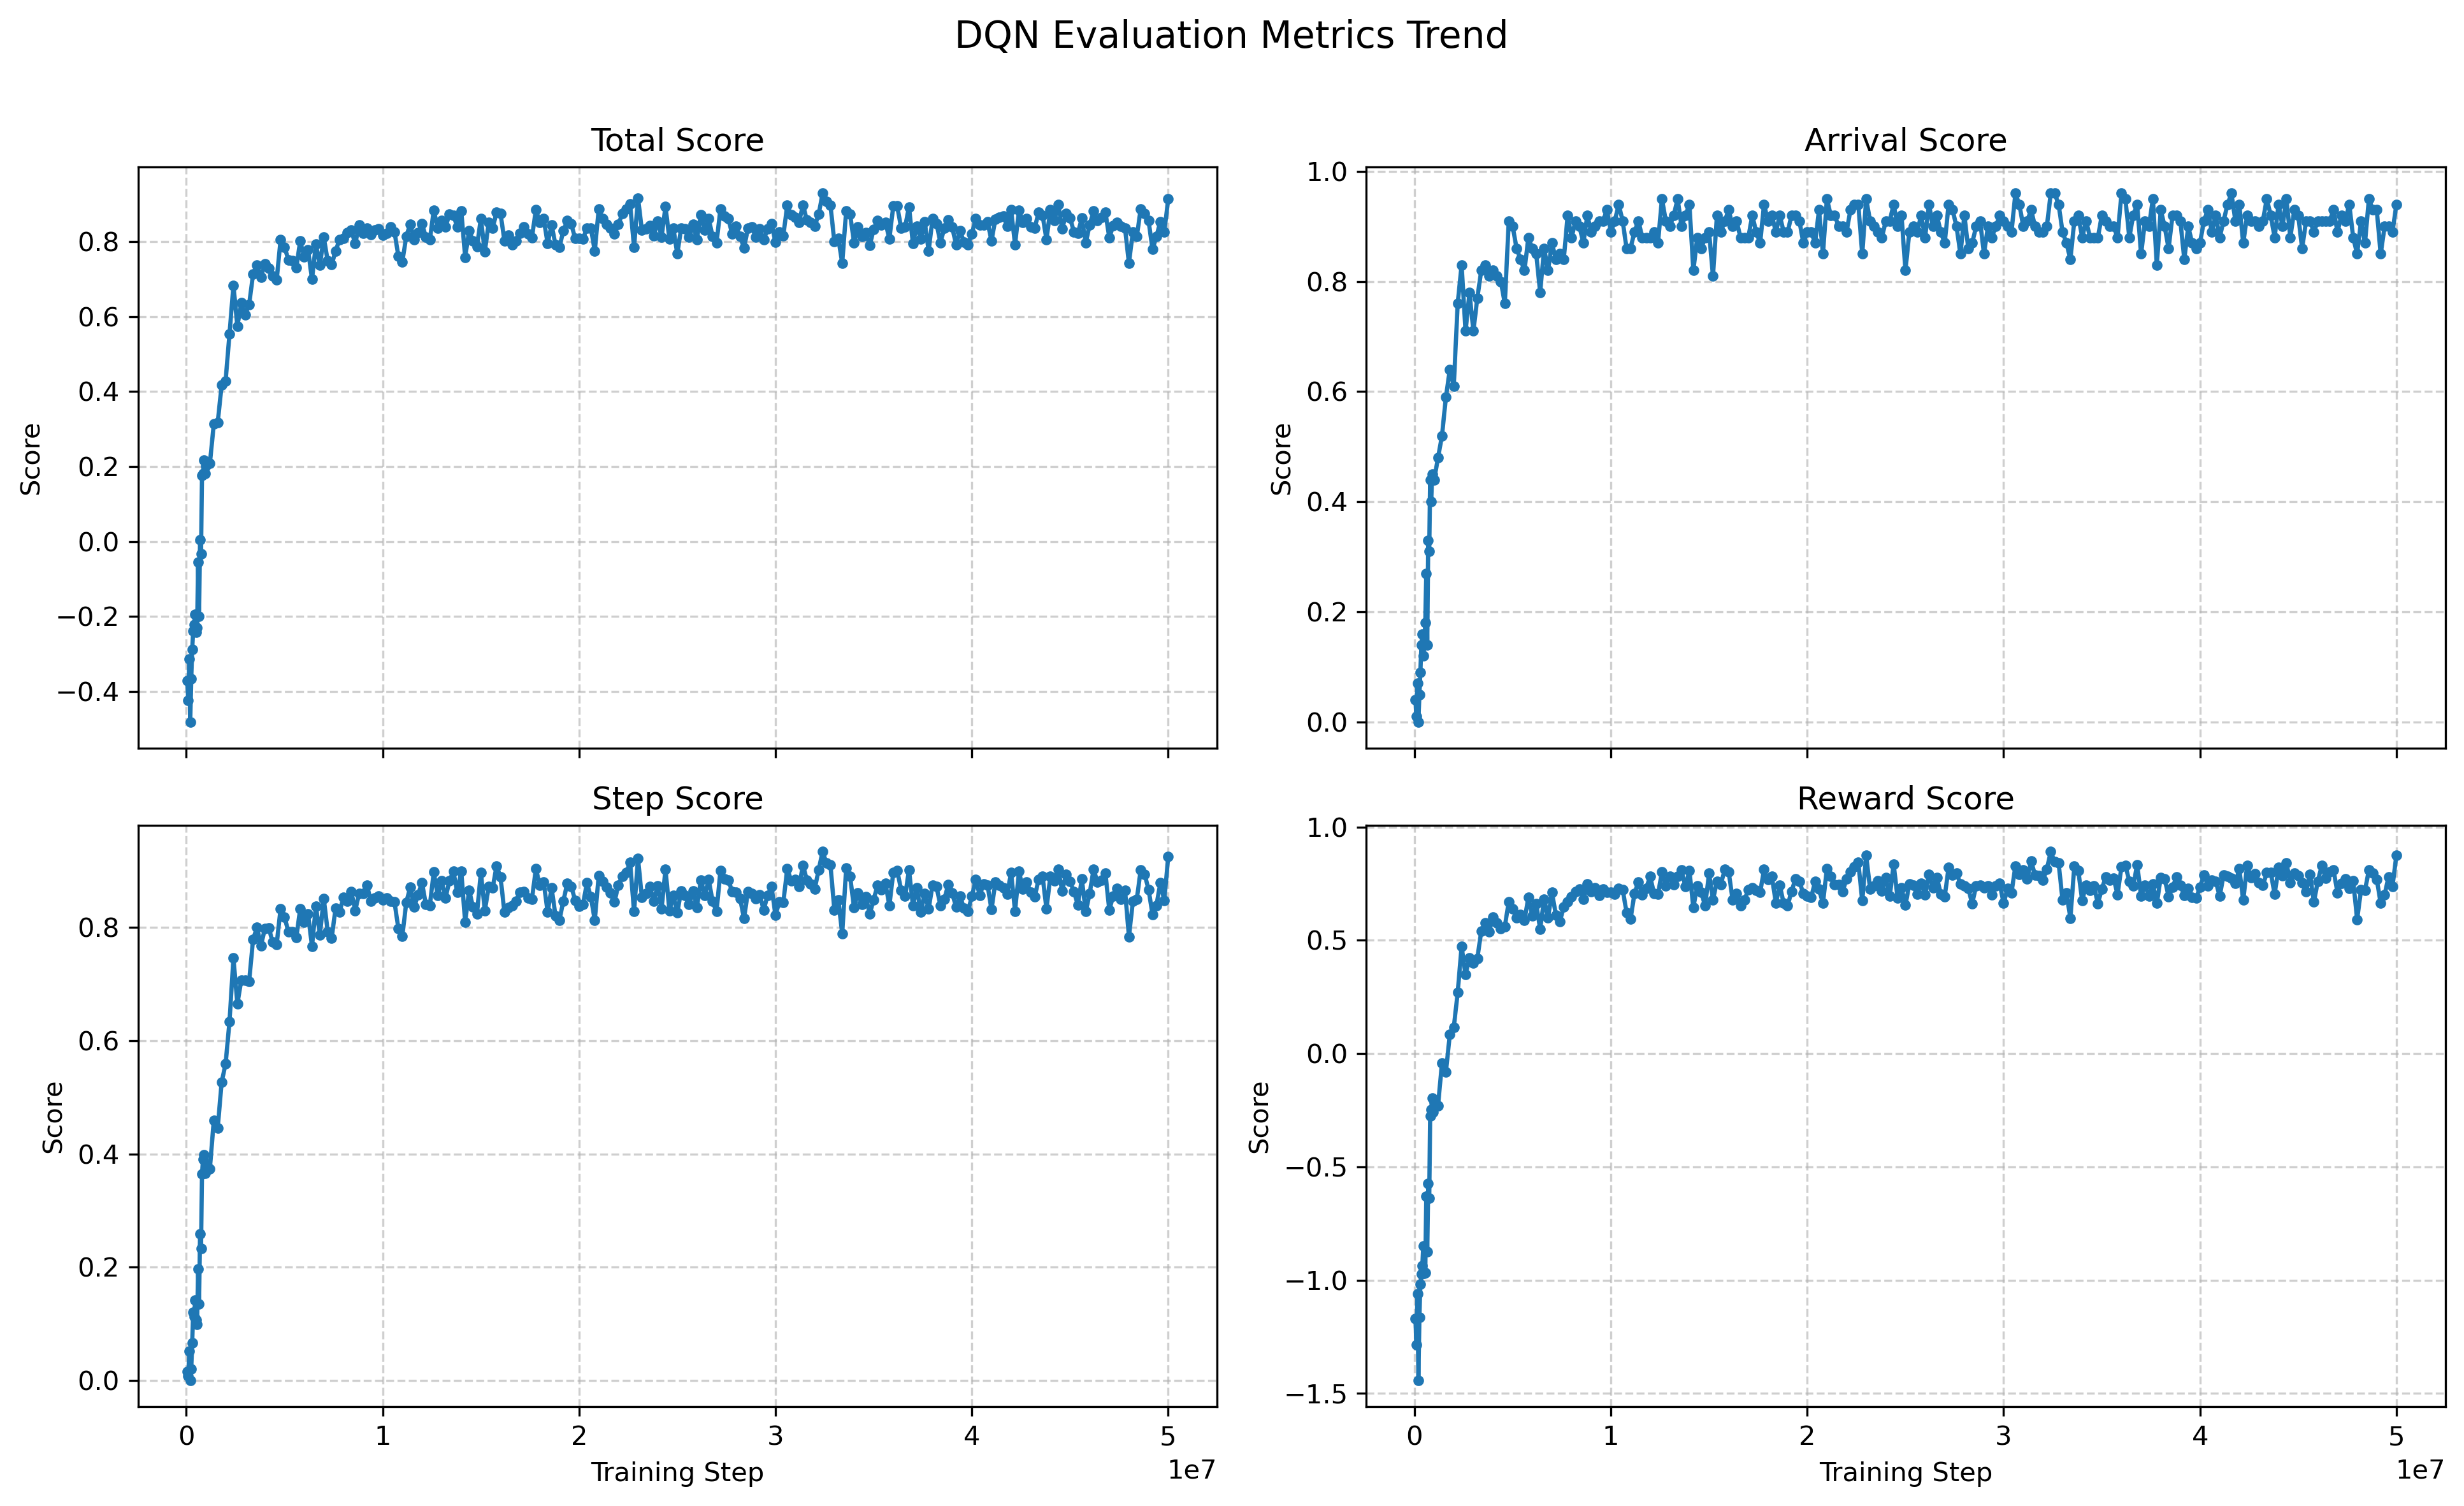
\includegraphics[width=0.7\textwidth]{figures/DQN_metrics_trend.png}
  \caption{DQN算法到达率、平均每回合步数和平均每回合奖励的训练趋势展示}
  \label{fig:dqn-showcase}
\end{figure}

从结果上看，DQN 在训练初期的探索波动相对明显，但由于离散动作空间的约束，整体收敛过程较为平稳，适合作为与连续控制算法对比的基础模型。其不足也较为直观：离散化动作会限制轨迹平滑性，机器人在转向和减速时难以形成更细粒度的控制，因此在复杂场景中的最终路径质量通常不及连续动作算法。

在训练初期（约 $0$ 至 $0.5 \times 10^7$ 步），各项指标均呈现出明显的爆发式增长。这表明智能体（Agent）在经验回放机制（Experience Replay）的作用下，能够迅速从随机探索中学习到有效策略。在 $1 \times 10^7$ 步之后，曲线进入平稳期，总分（Total Score）稳定在 0.8 左右，到达率（Arrival Score）稳定在 0.9 左右，证明算法具备良好的收敛性。

综合四项指标来看，DQN 算法在该任务场景下表现优异。步数得分（Step Score）与总分的高度一致性暗示了智能体在保证成功率的同时，也在不断优化路径或决策序列的效率。实验结果表明，所设计的奖励函数与状态空间能够引导模型学习到最优策略。

\section{SAC算法调试与ASL框架接入}
\subsection{SAC算法实现与连续动作训练}
与 DQN 相比，SAC 直接输出连续的线速度与角速度，更适合描述机器人在路径规划中的真实运动学约束，也更容易得到平滑自然的行驶轨迹。\cite{chen2022deep}本文采用 Actor-Critic 结构对策略和价值函数进行联合建模，其中 Actor 负责给出随机策略分布，Critic 则通过双 Q 网络对动作质量进行估计，从而缓解 Q 值高估带来的训练偏差。

在工程实现上，SAC 的训练流程与本文引入的 ASL（Actor-Learner-Sharer）框架高度适配。Actor 侧持续与环境交互并向共享经验池写入轨迹数据，Learner 则从经验池中批量采样并执行参数更新，这种解耦方式有效减少了采样与训练之间的相互阻塞，提高了系统吞吐量。对于路径规划任务而言，这一结构的实际意义在于：机器人可以在高频交互中持续积累有效样本，而网络更新则在后台稳定进行，最终形成更高的样本利用效率和更平滑的收敛曲线。

调试过程中，SAC 的主要问题集中在探索阶段的随机性偏强，以及熵系数和更新节奏对收敛速度的敏感性。为此，本文在训练中对动作幅值、奖励尺度以及更新频率进行了统一约束，使策略在前期保持足够探索、后期逐步转入稳定利用。整体来看，SAC 相比 DQN 在连续控制精度和路径平滑性上具有更明显的优势，是本文后续引入 Transformer 时采用的基础骨架。

但由于SAC 训练相对于DQN所需训练时间更长，训练效率受限于单进程的采样与更新模式，本文在后续章节中引入了 ASL 分布式训练架构，以实现更高效的并行加速。

\subsection{分布式训练架构设计--Actor-Learner-Sharer模型}
\label{sec:shared_data_module}

\subsubsection{模块设计背景与目标}

在传统的单进程强化学习算法中，环境交互（数据采样）与神经网络更新（梯度下降）通常是串行执行的。这种同步阻塞的模式导致底层硬件算力无法得到充分利用，极大限制了算法的采样效率与收敛速度。因此需要分布式训练架构来解耦数据采集与模型训练的物理进程，从而实现真正意义上的并行加速。

\begin{tikzpicture}[
    % 定义通用样式
    task/.style={rectangle, draw=black, fill=blue!40, minimum width=2.5cm, minimum height=0.8cm, align=center},
    subtask/.style={rectangle, draw=black, fill=blue!40, minimum width=1.4cm, minimum height=0.6cm, align=center},
    cnode/.style={rectangle, draw=black, dashed, fill=gray!10, rounded corners=2pt, minimum width=2.5cm, minimum height=1.2cm, align=center},
    output/.style={rectangle, draw=black, fill=green!40!lime!60, minimum width=2.5cm, minimum height=0.6cm, align=center},
    % 定义箭头样式
    myarrow/.style={-{Stealth[scale=1.2]}, line width=3pt, draw=blue!40!gray}
]

% ====================
% (a) 单计算节点
% ====================
\node[task] (taskA) {任务};
\node[cnode, below=1cm of taskA] (nodeA) {计算节点};
\node[output, below=1cm of nodeA] (outA) {输出};

\draw[myarrow] (taskA) -- (nodeA);
\draw[myarrow] (nodeA) -- (outA);

\node[below=0.3cm of outA, font=\sffamily] {(a) 单计算节点};


% ====================
% (b) 分布式多计算节点
% ====================
\begin{scope}[xshift=8cm] % 将右侧图形整体向右平移
    
    % 上层：子任务
    \node[subtask] (sub2) {子任务2};
    \node[subtask, left=0.1cm of sub2] (sub1) {子任务1};
    \node[subtask, right=0.1cm of sub2] (sub3) {子任务3};

    % 中层：计算节点
    \node[cnode, below=1cm of sub2] (node2) {计算节点2};
    \node[cnode, left=0.3cm of node2] (node1) {计算节点1};
    \node[cnode, right=0.3cm of node2] (node3) {计算节点3};

    % 下层：输出
    \node[output, below=1cm of node2, minimum width=3cm] (outB) {输出};

    % 绘制连线
    \draw[myarrow] (sub1.south) -- (node1.north);
    \draw[myarrow] (sub2.south) -- (node2.north);
    \draw[myarrow] (sub3.south) -- (node3.north);

    \draw[myarrow] (node1.south) -- (outB.north west);
    \draw[myarrow] (node2.south) -- (outB.north);
    \draw[myarrow] (node3.south) -- (outB.north east);

    \node[below=0.3cm of outB, font=\sffamily] {(b) 分布式多计算节点};

\end{scope}

\end{tikzpicture}
为了解决上述计算瓶颈和资源闲置问题，本研究提出了一个演员-学习者分布式训练架构。 该架构在物理过程层面上深刻地解耦了环境交互（数据采样）和模型更新（参数学习）。 因此，计算瓶颈被打破，资源利用率和训练吞吐量都得到了改善。 该架构由三个核心组成部分组成。

\begin{enumerate}
\item Actor（演员采样器）：演员负责与环境的高频交互。 它执行当前收集经验轨迹的政策。 单步转换通常记录为$(s_t, a_t, r_t, s_{t+1})$。 由于模拟环境执行和逻辑推理是CPU密集型任务，Actors可以像许多独立进程或容器一样并行部署。 每个演员实例在独立的模拟环境中运行。 收集的数据异步写入中央体验池或流式传输到学习者。

\item Learner（学习者）：学习者专注于优化神经网络参数。 它从经验池中提取迷你批次数据，并根据相应的损失函数（如SAC中的Actor-Critic损失或DQN中的TD误差）执行反向传播。 学习者是一项 GPU/TPU 密集型任务，因此它专门占用加速的硬件资源。 它不需要等待环境交互的物理时间延迟。 因此，学习者实现了非常高的样本处理效率和梯度更新速度。

\item Sharer（参数分配器）：Sharer通常作为参数服务组件在大规模集群中独立部署。 它的主要职责是全球网络权重的版本管理和分配。 当许多演员同步并拉取最新参数时，这种设计减少了学习者计算和网络带宽的I/O瓶颈。 通过高效的参数同步，共享器确保每个演员部署的策略不会变得过时。 它还严格控制非策略算法中的分布偏差。

\end{enumerate}

\subsubsection{共享数据中心的设计}
为了实现跨流程和异构硬件（CPU和GPU）的高效协作，本节基于ColorDynamic导航系统\cite{colordynamic}中的相关工作，设计和实现一个高性能共享数据中心模块（\texttt{共享数据模块}）。 该模块充当“中央物流枢纽”，连接数据收集端和模型训练端。 系统将此模块直接部署在主存储器（RAM）中，以完全消除高频通信造成的I/O瓶颈。 共享内存机制用于实现较快的进程间交互。 该模块主要有两个核心功能：
\begin{enumerate}

\item 该模块构建高速数据管道。 它接收来自多个演员的并发经验写入，而不会阻止。 同时，它提供了高通量随机批次采样。 这种抽样支持学习者的快速迭代。

\item 异步状态同步由模块实现。 该模块充当策略网络参数的高速寄存器。 学习者完成渐变更新后，模块会协调参数的异步调度。 在开始新回合之前，演员可以以非阻塞的方式拉动参数。

\end{enumerate}

共享数据模块充当中央物流枢纽。 它连接了数据收集端和模型训练端。 为了消除I/O瓶颈，系统将此模块部署在主存储器（RAM）中。 这里使用共享记忆体机制来实现快速程序间通讯。 该模块的数据流转架构如图\ref{fig:shared_data_arch}所示：

\begin{figure}[H]
    \centering
\begin{tikzpicture}[
    % ==== 定义通用样式 ====
    % 基础节点样式
    basebox/.style={
        rectangle, draw=black!60, thick, rounded corners=6pt, 
        align=center, minimum height=1.8cm, text=black,
        drop shadow={opacity=0.15, shadow xshift=1.5mm, shadow yshift=-1.5mm}
    },
    % 特定节点样式（带微渐变）
    buffer/.style={basebox, top color=blue!5, bottom color=blue!15, minimum width=4.8cm},
    register/.style={basebox, top color=orange!5, bottom color=orange!15, minimum width=4.8cm},
    actorbox/.style={basebox, top color=green!5, bottom color=green!15, minimum width=5cm},
    learnerbox/.style={basebox, top color=red!5, bottom color=red!15, minimum width=5cm},
    % 箭头样式
    data_arrow/.style={-{Stealth[scale=1.2]}, line width=1.5pt, draw=blue!70!gray, text=black!80},
    weight_arrow/.style={-{Stealth[scale=1.2]}, line width=1.5pt, draw=orange!80!red, text=black!80},
    % 共享内存背景样式
    shared_mem/.style={
        rectangle, draw=black!40, dashed, thick, rounded corners=10pt, 
        fill=gray!8, inner sep=18pt
    }
]

% ==== 1. 定义顶部节点 (Shared Memory 内部) ====
\node[buffer] (buffer) {
    \textbf{向量化环形经验池} \\
    \fontsize{9pt}{10pt}\selectfont \sffamily (Ring Replay Buffer) \\
    \vspace{2pt}
    \fontsize{8pt}{9pt}\selectfont \ttfamily \color{black!70} [s, a, r, s', dw] \sffamily 异构张量存储
};

\node[register, right=2.5cm of buffer] (register) {
    \textbf{模型参数寄存器} \\
    \fontsize{9pt}{10pt}\selectfont \sffamily (Actor Policy Weights) \\
    \vspace{2pt}
    \fontsize{8pt}{9pt}\selectfont \ttfamily \color{black!70} [actor\_param] \sffamily 字典状态字典
};

% ==== 2. 绘制共享数据中枢背景框 ====
\begin{scope}[on background layer]
    \node[shared_mem, fit=(buffer) (register)] (shared) {};
    % 背景框的标题
    \node[anchor=south, font=\bfseries\sffamily\large, text=black!80, yshift=4pt] 
        at (shared.north) {Shared Data 通信中枢 (主内存 RAM)};
\end{scope}

% ==== 3. 定义底部节点 ====
\node[actorbox, below=3.5cm of buffer] (actor) {
    \textbf{Actor 进程} \small (数据采集端) \\
    \vspace{2pt}
    \fontsize{9pt}{10pt}\selectfont \sffamily \color{black!70} (运行于 CPU 或 推理 GPU)
};

\node[learnerbox, below=3.5cm of register] (learner) {
    \textbf{Learner 进程} \small (模型训练端) \\
    \vspace{2pt}
    \fontsize{9pt}{10pt}\selectfont \sffamily \color{black!70} (运行于 高性能 GPU)
};

% ==== 4. 绘制数据流转箭头 ====

% (1) Actor -> Buffer (写入经验)
\draw[data_arrow] (actor.north) -- (buffer.south) 
    node[midway, left=4pt, font=\sffamily\small] {写入转移经验};

% (2) Learner -> Register (更新权重)
\draw[weight_arrow] (learner.north) -- (register.south) 
    node[midway, right=4pt, font=\sffamily\small] {更新权重};

% (3) Buffer -> Learner (采样批次数据 - 交叉线)
% 使用 pos 参数调整文字位置，并添加白色背景避免线条穿过文字
\draw[data_arrow] (buffer.315) -- (learner.135) 
    node[pos=0.25, right=4pt, font=\sffamily\small, fill=white, inner sep=2pt, rounded corners=2pt] {采样批次数据};

% (4) Register -> Actor (拉取最新权重 - 交叉线)
\draw[weight_arrow] (register.225) -- (actor.45) 
    node[pos=0.25, left=4pt, font=\sffamily\small, fill=white, inner sep=2pt, rounded corners=2pt] {拉取最新权重};

\end{tikzpicture}
\caption{分布式 Actor-Learner 共享数据流转架构图}
\label{fig:shared_data_arch}
\end{figure}

\subsubsection{核心数据结构设计}
为了满足大规模分布式强化学习中并发读写以及异构设备协作的需求，本模块在设计低级数据结构时遵循两个核心原则。 第一个原则是矢量化存储，用于支持并行采样。 第二个原则是具有异构装置感知的透明映射，它消除了资料流中的物理瓶颈。

\paragraph{矢量化环缓冲区}

在此架构中，演员端并行部署$N$独立模拟环境以进行同步采样。 传统的二维体验池$(Max\_Size, Feature\_Dim)$需要在写入之前将$N$环境中的数据依次串联。 此操作带来了高频列表操作和内存重排开销。 为了解决这个问题，该模块将体验重放池升级为三维张量结构$\mathcal{D} \in \mathbb{R}^{Max\_Size \times N \times State\_Dim}$。 有了这种结构，来自$N$环境的采样数据可以在低级原子写入矩阵块。 因此，避免了序列化和重新索引的计算浪费。

同时，使用环形缓冲覆盖机制来防止内存使用量的无限增长。 系统保留一个循环写入指针$ptr$。 每次写入新数据时，指针都会自动增加。 当$ptr$达到$Max\_Size$时，指针通过模操作$ptr \leftarrow ptr \bmod Max\_Size$包裹回缓冲区的开头，新样本覆盖最古老的数据。 这种设计确保数据保持最新，这意味着学习者从相对新鲜的过渡中抽样。 它还将峰值内存使用量严格锁定在预先分配的上限，从而避免了动态扩展的GC延迟。

\paragraph{三设备内存映射}

在实际部署中，数据移动涉及三种类型的计算设备。 这些是演员端推理设备（CPU或推理GPU，表示为$A\_dvc$）、中央存储设备（主存储RAM，表示为$B\_dvc$）和学习者端训练设备（高性能GPU，表示为$L\_dvc$）。 如果在数据插入和采样的每个步骤中手动管理这些设备之间的张量传输，这会导致繁重的代码耦合和不可预测的内存碎片化。

为此，本模块在初始化时显式配置这三类设备标识，在执行 $\texttt{Add}()$ 与 $\texttt{Sample}()$ 等核心操作时自动调用 PyTorch 的设备转移接口（如 $\texttt{.to}(device)$）。具体地，当 Learner 调用 $\texttt{Sample}()$ 方法时，系统先从主内存批量读取数据，随后在返回前自动将其转移至 $L\_dvc$，使调用方无需感知底层的设备寻址细节。

\begin{algorithm}
\caption{共享数据中枢的异构张量流转与自旋锁控制伪代码}
\label{alg:shared_data}
\textbf{输入}: 采集端设备 $A\_dvc$ (CPU), 训练端设备 $L\_dvc$ (GPU), 经验池容量 $Max\_Size$, 批次大小 $B$\\
\textbf{初始化}: 
\begin{itemize}
    \vspace{-0.2cm}
    \item 预分配主存 ($RAM$) 经验池张量 $\mathcal{D} \in \mathbb{R}^{Max\_Size \times N \times State\_Dim}$
    \item 初始化自旋锁状态矩阵 $busy \leftarrow [\text{False}, \text{False}]$
    \item 队列写入指针 $ptr \leftarrow 0$
\end{itemize}
\vspace{-0.2cm}
\begin{algorithmic}[1]
\Function{Add}{$transition\_data$} \Comment{由 Actor 并发调用，位于 $A\_dvc$}
    \While{$busy[1] == \text{True}$} \Comment{轻量级自旋锁等待}
        \State \text{Pass} 
    \EndWhile
    \State $busy[1] \leftarrow \text{True}$ \Comment{获取经验池锁}
    \State $\mathcal{D}[ptr] \leftarrow transition\_data$ \Comment{数据存入主内存}
    \State $ptr \leftarrow (ptr + 1) \pmod{Max\_Size}$ \Comment{环形队列覆写机制}
    \State $busy[1] \leftarrow \text{False}$ \Comment{释放锁}
\EndFunction

\State
\Function{Sample}{} \Comment{由 Learner 高频调用，意图用于 $L\_dvc$}
    \While{$busy[1] == \text{True}$} 
        \State \text{Pass} 
    \EndWhile
    \State $busy[1] \leftarrow \text{True}$
    \State $batch \leftarrow \text{RandomSelect}(\mathcal{D}, B)$ \Comment{从主内存抽取小批量数据}
    \State $busy[1] \leftarrow \text{False}$
    
    \State $batch\_L \leftarrow \text{batch.to}(L\_dvc)$ \Comment{\textbf{底层隐式设备映射}}
    \State \Return $batch\_L$ \Comment{返回的张量已原生驻留于 GPU}
\EndFunction
\end{algorithmic}
\end{algorithm}

\subsubsection{并发控制和轻量级读写锁定机制}

在多进程共享内存架构中，并发访问冲突限制了系统性能。 假设学习者写入参数寄存器，同时演员尝试读取该参数。 然后张量内存可能会损坏。 传统的全球互斥带来了更严重的问题。 它迫使所有竞争线程进入阻止状态，并触发昂贵的内核级上下文切换。 对于纳秒级别的张量访问操作，这种成本非常高。

为了解决这个问题，系统使用精细的旋转锁机制，而不是系统级锁。 核心思想是保持状态向量$\texttt{busy} \in \{\text{False}, \text{False}\}$。 在这里，$\texttt{busy}[0]$保护模型参数寄存器的读写，$\texttt{busy}[1]$保护体验池的读写。 这种精细的分离允许系统独立控制数据域和权重域中的争用。 因此，全局锁阻塞的概率大大降低。

更重要的是，当一个进程发现目标锁被占用时，它不会暂停和等待（暂停费用约为$\sim 100\,\mu s$）。 相反，它进入一个紧密的自旋轮询状态，周期约为$\sim 10^{-4}\,s$。 张量操作通常非常短，持续时间不到1毫秒。 对于短期轮询，成本远远低于唤醒线程的延迟。 因此，系统实现了阻塞等待比阻止更好的情况。 与此同时，轮询确实消耗了CPU周期。 但学习者和演员在不同的物理核心上运行。 因此，这种消耗并不能与GPU计算资源竞争。 相反，它充分利用了多核计算平面。

当两端的进程争夺相同的锁时，例如，当演员和学习者都访问体验池时，旋转锁机制会导致未能获取锁的进程在\texttt{while True}循环中进入高频轮询状态。 在这种状态下，它保持高频率的轮询（$10^{-4}$秒级），而不是暂停和等待。 张量转移操作需要很少的时间。 因此，这种短期轮询机制可以确保数据安全，同时保持低等待开销。

\begin{figure}[http]
  \centering
  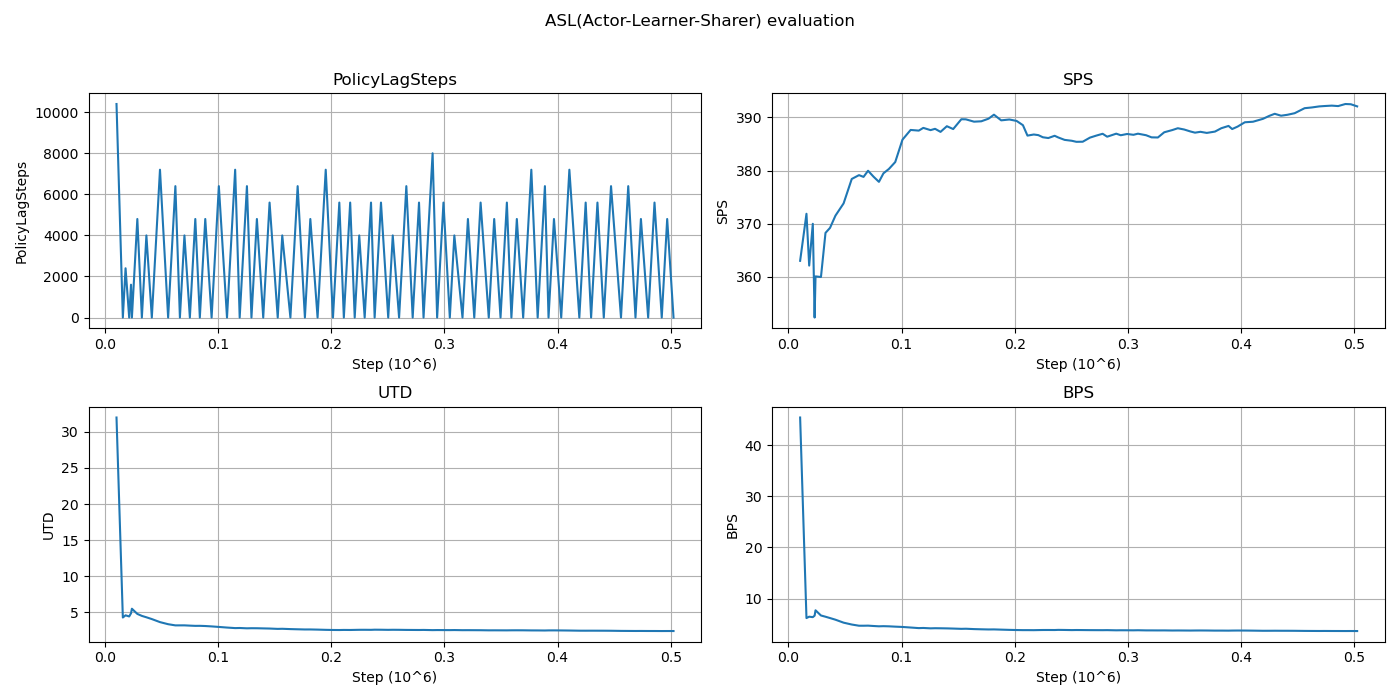
\includegraphics[width=0.9\textwidth]{figures/ASL_analysis.png}
  \caption{ASL架构性能分析}
  \label{fig:ASL-analysis}
\end{figure}
在分布式强化学习训练中，系统吞吐量、资源利用率与组件通信延迟是评估架构有效性的核心指标。图\ref{fig:ASL-analysis}给出了 Actor-Learner-Sharer（ASL）架构在 50 万步（$0.5 \times 10^6$ steps）训练周期内的性能曲线。结合曲线形态，可归纳为以下三点：
\begin{enumerate}
    \item 高效和分离并发吞吐量（SPS \& BPS 分析）

    ASL架构的主要优势来自于通过共享器将数据采样（演员）和梯度计算（学习者）的物理和逻辑解耦合。 数据采样率（SPS - 每秒步数）如图所示。 SPS曲线在训练开始时短暂热身后迅速攀升，然后在380到390之间保持稳定。 这种行为表明，演员流程组可以持续高效地与环境互动。 SPS的稳步和逐渐增加也表明，环境重置或缓存机制在长期运行中效果良好。 没有观察到阻塞或内存泄漏等性能下降。 对于每秒批次（BPS），学习者的BPS曲线在探索期的早期训练中很高。 然后它迅速下降，在4点左右保持稳定。 SPS和BPS独立稳定运行这一事实提供了强有力的证据。 ASL架构成功地打破了传统单过程RL中看到的“采样然后训练，训练后采样”的同步效应。 它还实现了CPU（环境推理）和GPU（梯度反向传播）计算能力的全负载管道操作。

    \item 稳定数据更新率（UTD分析）

    UTD（更新与数据比率）定义了网络更新与环境交互步骤数量的比率。 它是控制强化学习训练节奏的关键超参数。 如图所示，UTD曲线与BPS曲线密切匹配。 它起初急剧下降，然后在保持较低，大约2到3。 这种低且稳定的UTD设置可确保学习者不会因为过度使用旧数据而过度拟合或高估 Q 值。 与此同时，演员不断注入高新鲜度的数据，以保持探索和开发之间的平衡。

    \item 异步通信和容忍延迟（PolicyLagSteps分析）

    政策延迟是衡量分布式架构中通信开销和政策陈旧性的最重要指标。 它记录了行为者当前使用的抽样策略落后于学习者最新政策的步数。

\end{enumerate}

\begin{figure}[http]
  \centering
  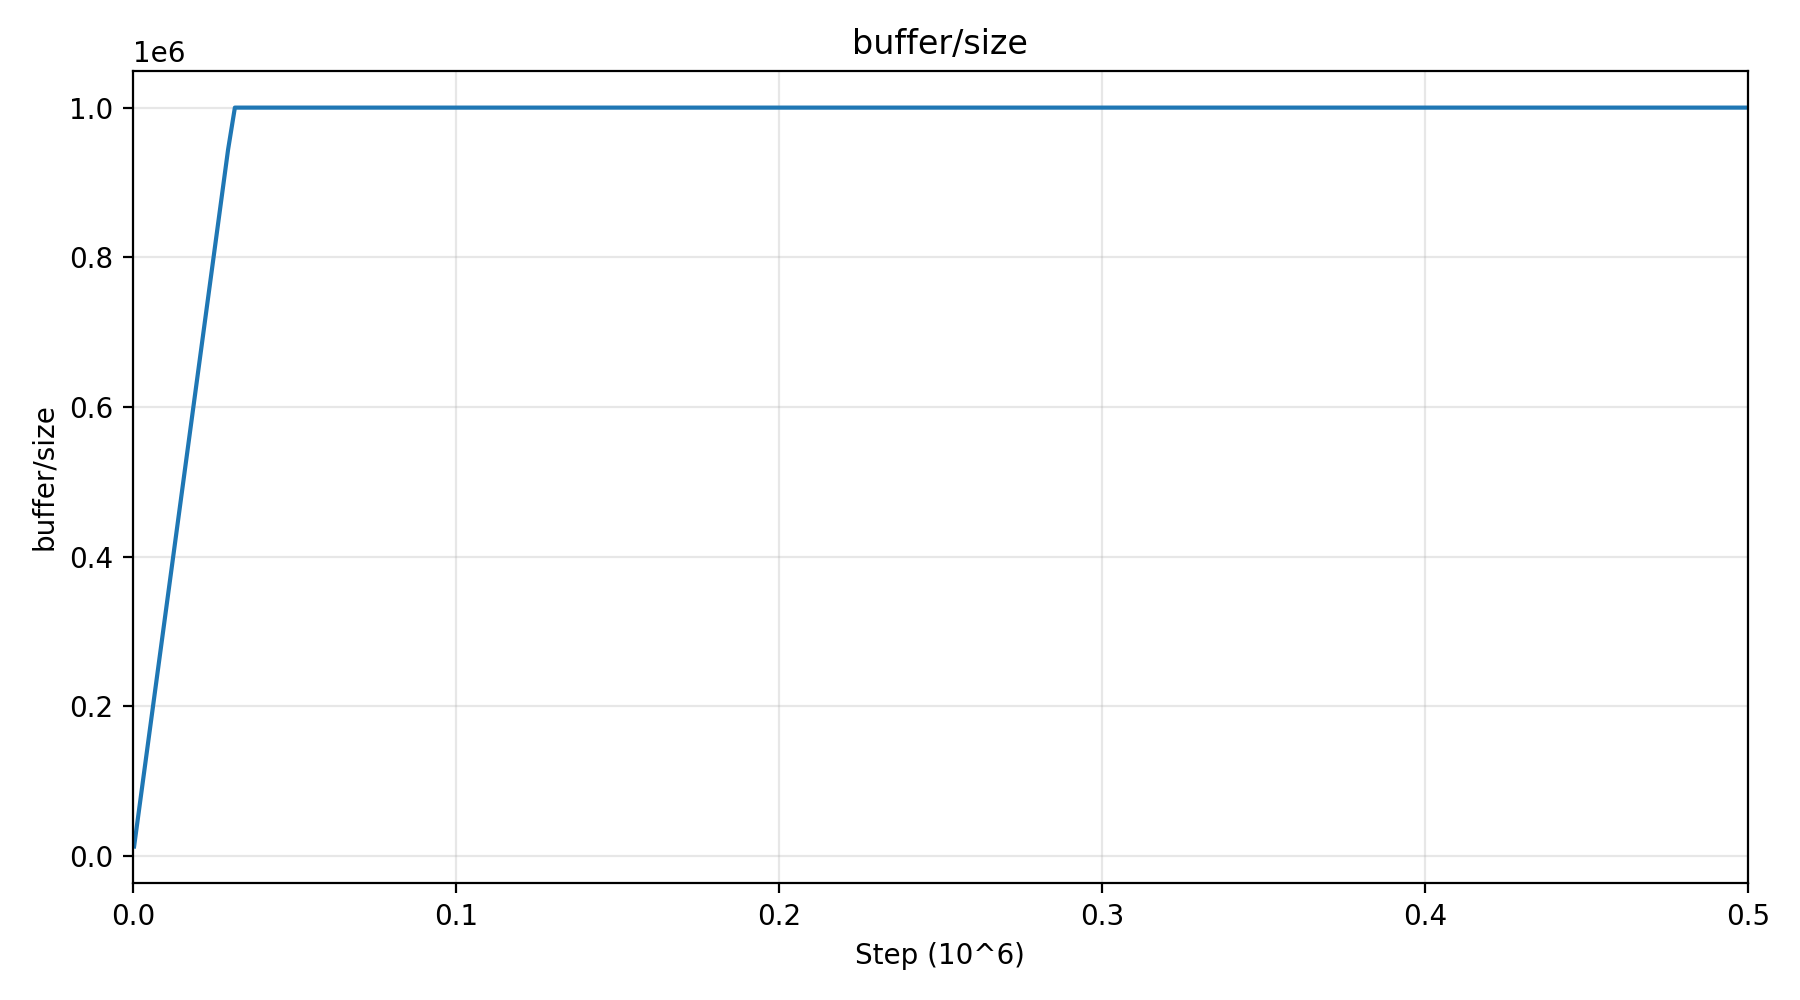
\includegraphics[width=0.9\textwidth]{figures/buffer.png}
  \caption{ASL架构训练时共享数据中枢的经验池占用率分析}
  \label{fig:buffer-analysis}
\end{figure}
由图\ref{fig:buffer-analysis} 可见，ASL 架构的共享数据中枢在训练过程中表现出极高的稳定性与效率：在横轴（Step）的最左侧，紫线几乎是垂直向上飙升的。这表明系统在训练初期就迅速填满了经验池，达到了预设的 100 万条转移数据的容量上限。随后，经验池的占用率曲线趋于平坦，稳定在 100\% 的水平，说明系统成功实现了环形覆盖机制，同时侧面印证了ASL系统的采集数据高效性。

\subsection{SAC算法评估分析}
\begin{figure}[http]
  \centering
  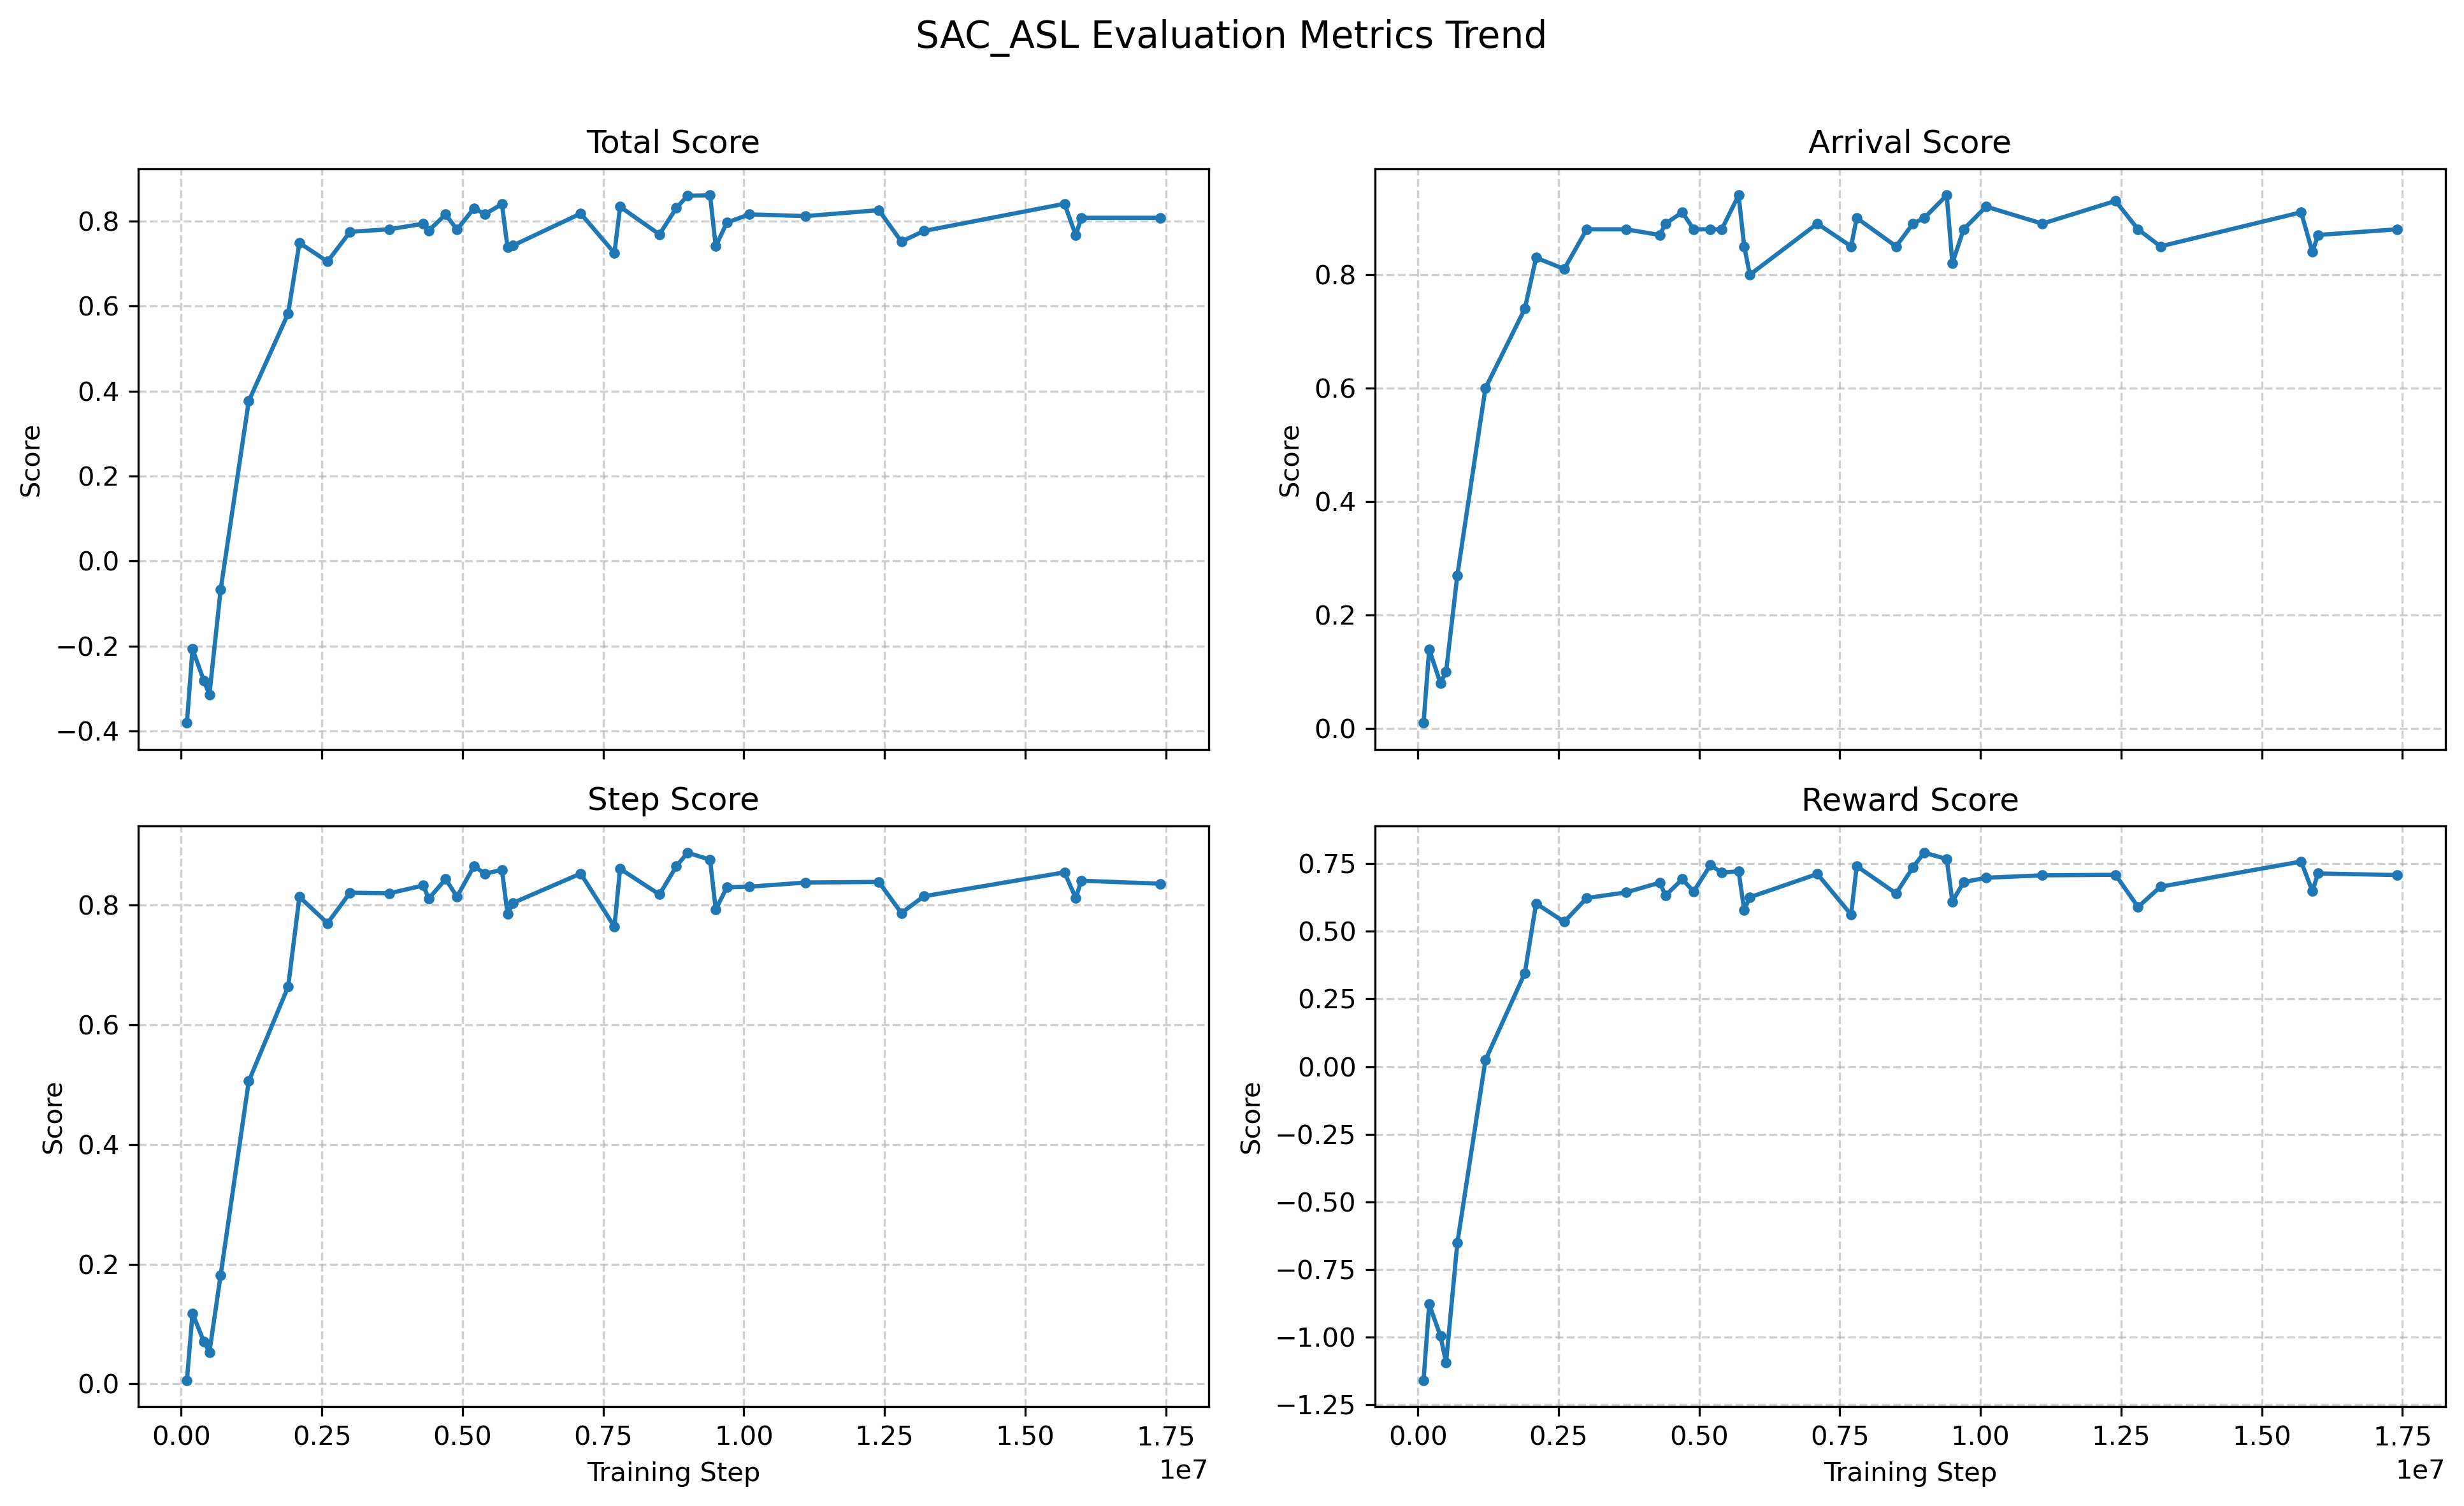
\includegraphics[width=0.9\textwidth]{figures/SAC_ASL_metrics_trend.png}
  \caption{SAC算法到达率、平均每回合步数和平均每回合奖励的训练趋势展示}
  \label{fig:sac-showcase}
\end{figure}

与传统强化学习算法相比，SAC\_ASL 表现出了极其优异的起步学习能力。在训练的极初期（约 $0$ 至 $0.25 \times 10^7$ 步），所有四项指标均呈现出几乎垂直的陡峭上升趋势。这表明该算法能够更高效地利用收集到的样本数据，在极短的探索期内便构建出了高质量的初始策略框架，大幅缩短了模型预热时间。

观察收敛后的曲线（$0.5 \times 10^7$ 步之后），可以发现指标在高位维持整体稳定的同时，伴有偶尔的局部下探（例如在约 $0.6 \times 10^7$ 和 $1.3 \times 10^7$ 步处）。这种现象高度符合 SAC 算法体系的特征：其内建的最大熵强化学习框架促使智能体在利用已知最优策略的同时，始终保持一定程度的随机探索。这种机制虽然会导致分数的短暂波动，但有效防止了模型陷入局部最优解，并在遭遇性能波动后能够迅速自我修复回到高分基线，证明了策略具备极强的鲁棒性。

综合而言，SAC\_ASL 算法在该实验环境中不仅收敛速度极快，且最终能够收敛到一个具备极高成功率和高效执行能力的策略上，充分验证了该算法（或改进机制）在当前复杂任务场景下的有效性与先进性。

\section{TransSAC算法调试}
\subsection{TransSAC算法实现与时序上下文增强}
TransSAC 是本文在 SAC 基础上的进一步增强版本，其核心思想是利用 Transformer 对历史状态序列进行编码，从而弥补标准 SAC 对短期上下文建模不足的问题。对于路径规划任务而言，机器人当前时刻的观测往往无法完整反映动态障碍物的运动趋势，尤其是在障碍物连续移动、环境反馈具有滞后性的情况下，单帧状态输入很容易导致策略出现“看见当前、忽略趋势”的局限。Transformer 的引入正是为了解决这一问题。

在实现上，本文将近期若干步的状态特征拼接为序列输入，通过自注意力机制提取其中的关键时序依赖，再将增强后的上下文特征送入 SAC 的策略网络与价值网络。这样做的直接收益是，模型不仅能判断“此刻是否安全”，还能更早捕捉障碍物的运动方向和目标区域的变化趋势，从而在决策上表现出更强的前瞻性。相比普通 SAC，TransSAC 往往在训练初期就能形成更稳定的动作偏好，路径选择也更少出现反复修正。

从训练表现来看，TransSAC 的优势主要体现在样本效率和早期收敛速度上。虽然其网络结构更复杂、单步计算开销略高，但由于时序特征提取更充分，策略可以更快建立对环境动态的稳定认知，因此在相同训练轮数下通常能获得更高的到达率和更低的平均步数。也正因如此，本文将其作为与 SAC 并列的重点对比对象，用于验证 Transformer 在路径规划强化学习中的增益。

TransSAC 在 SAC 基础上引入 Transformer 编码器，使网络能够对历史状态序列进行时序建模。相比于逐帧处理，这一设计使模型能够捕捉环境动态的长期依赖，对于部分可观测环境（POMDP）下的路径规划任务尤为关键。本节介绍其核心架构与调试要点。

\subsubsection{TransSAC 网络结构}
\begin{figure}[htbp]
    \centering
    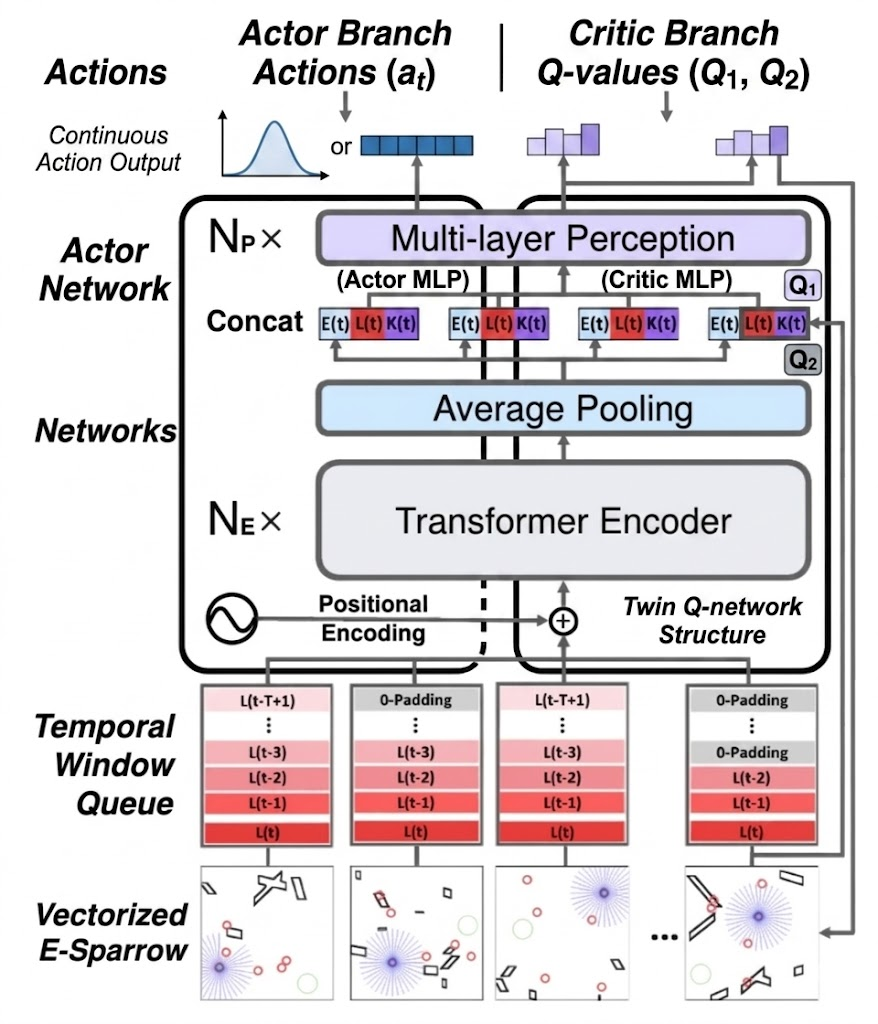
\includegraphics[width=0.5\textwidth,keepaspectratio]{figures/TransSAC_structure.png}
    \caption{TransSAC 网络结构}
    \label{fig:transSAC-structure}
\end{figure}

如图\ref{fig:transSAC-structure}所示，系统维护一个长度为 $T$ 的时序窗口队列，存储最近 $T$ 个时刻的向量化观测值 $\{L(t-T+1), \dots, L(t)\}$。TransSAC 的状态表示由这一时序窗口组成 $\mathbf{s}_t = \{l_{t-T+1}, \dots, l_t\}$。

特征提取过程定义如下：先通过位置编码（Positional Encoding）为序列添加时间信息，随后经 $N_E$ 层 Transformer 编码块进行自注意力编码，最后通过全局平均池化压缩为固定维度的特征向量：

\begin{equation}
    \mathbf{z}_t = \text{AvgPool}(\text{TransformerEnc}(\mathbf{s}_t + \text{PE}))
\end{equation}

其中，$\text{PE}$ 为位置编码，$\mathbf{z}_t \in \mathbb{R}^{d_{feat}}$ 为增强后的全局特征。

Actor 与 Critic 网络分别以 $\mathbf{z}_t$ 作为输入，输出为：

\begin{align}
    \pi(a_t|s_t) &= \mathcal{N}(\mu_{\theta}(\mathbf{z}_t), \sigma_{\theta}(\mathbf{z}_t)) \\
    Q_{\phi}(\mathbf{s}_t, a_t) &= \text{MLP}_{\phi}(\text{Concat}(\mathbf{z}_t, a_t))
\end{align}
Actor 网络经过 $N_P$ 层 MLP 后输出策略分布参数；Critic 包含两个独立的 Q 网络，以实现 SAC 的双采样机制并缓解 Q 值高估。
\subsubsection{时序特征提取的优势}
与标准 SAC 相比，TransSAC 在以下方面表现出优势：
\begin{enumerate}
    \item 动态环境感知：Transformer 的自注意力机制能够自适应地学习历史状态中的关键时间步，使模型对动态障碍物的运动轨迹形成更准确的预判。
    \item 降低路径抖动：时序上下文能够稳定策略的决策过程，避免单帧观测导致的前后不一致的动作选择。
    \item 提升样本效率：通过编码足够的历史信息，网络能够更快地学到有效策略，整体收敛速度超过逐帧处理的方案。
\end{enumerate}

\subsection{Transformer训练调试与超参数配置}
\begin{figure}[http]
    \centering
    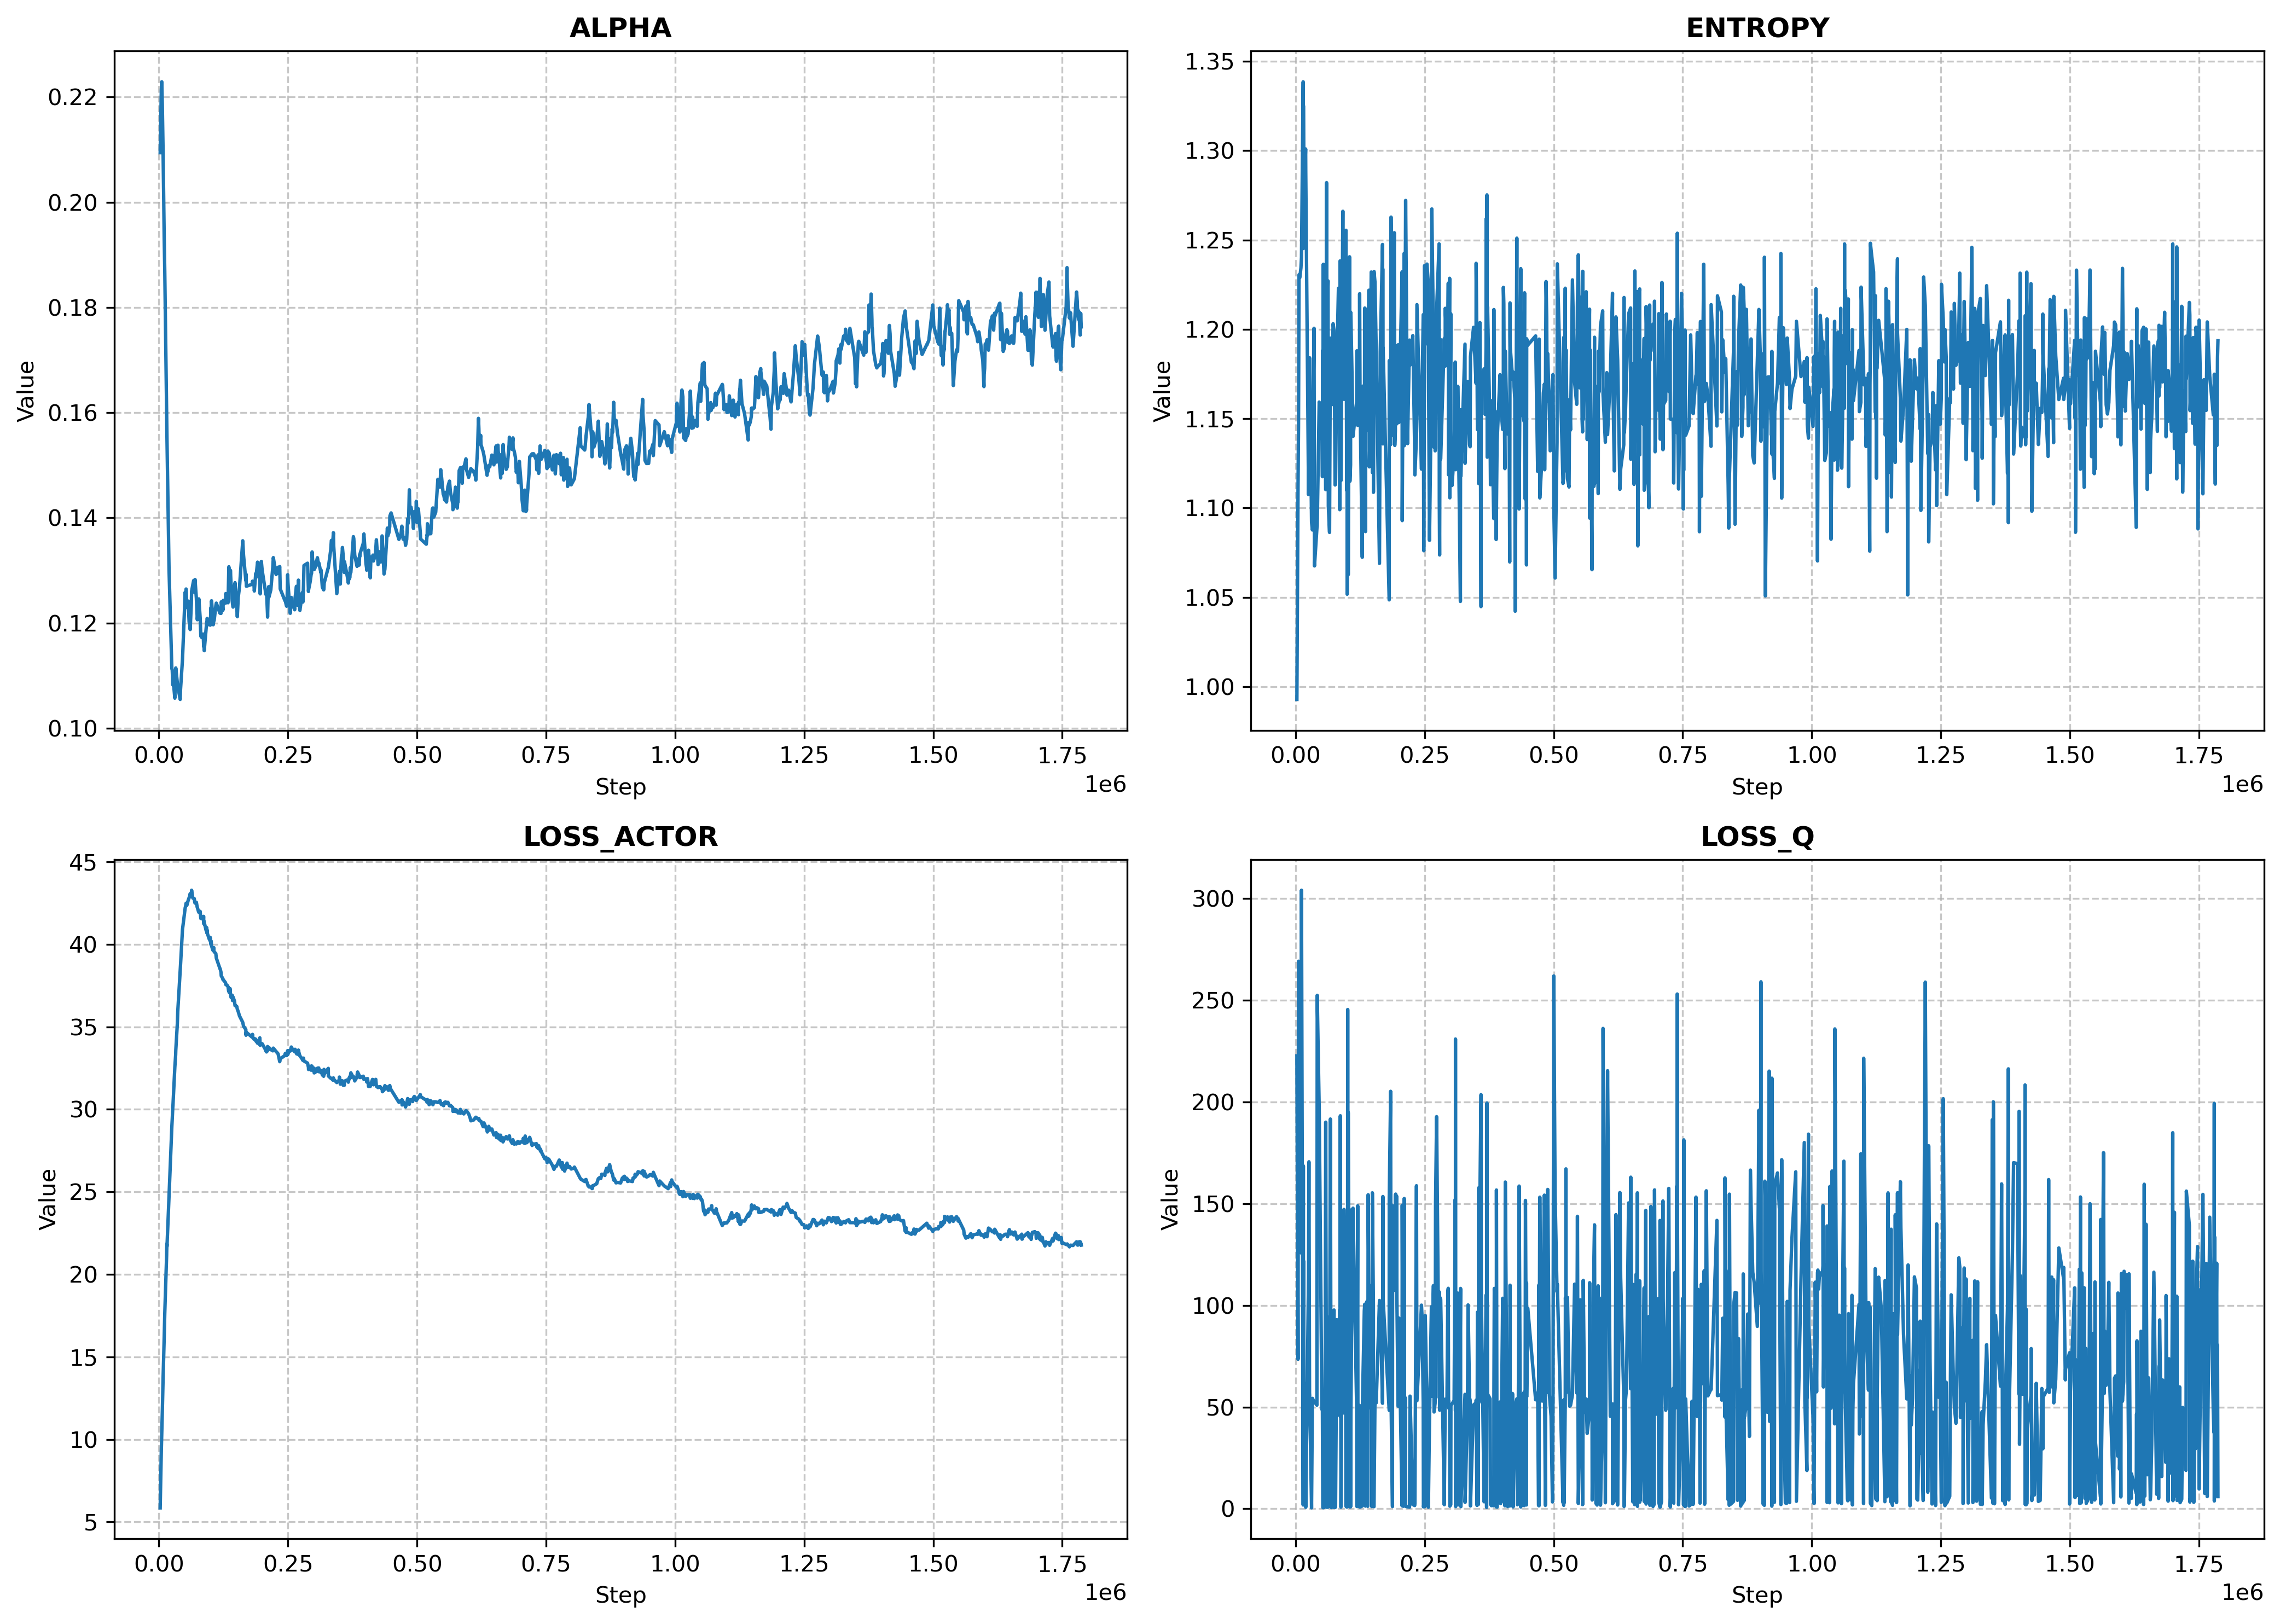
\includegraphics[width=0.9\textwidth,height=0.38\textheight,keepaspectratio]{figures/bad_transSAC/bad_transSAC_ASL_train_combined.png}
    \caption{TransSAC 训练中策略网络崩塌训练记录}
    \label{fig:transSAC-train-bad}
\end{figure}
\begin{figure}[http]
    \centering
    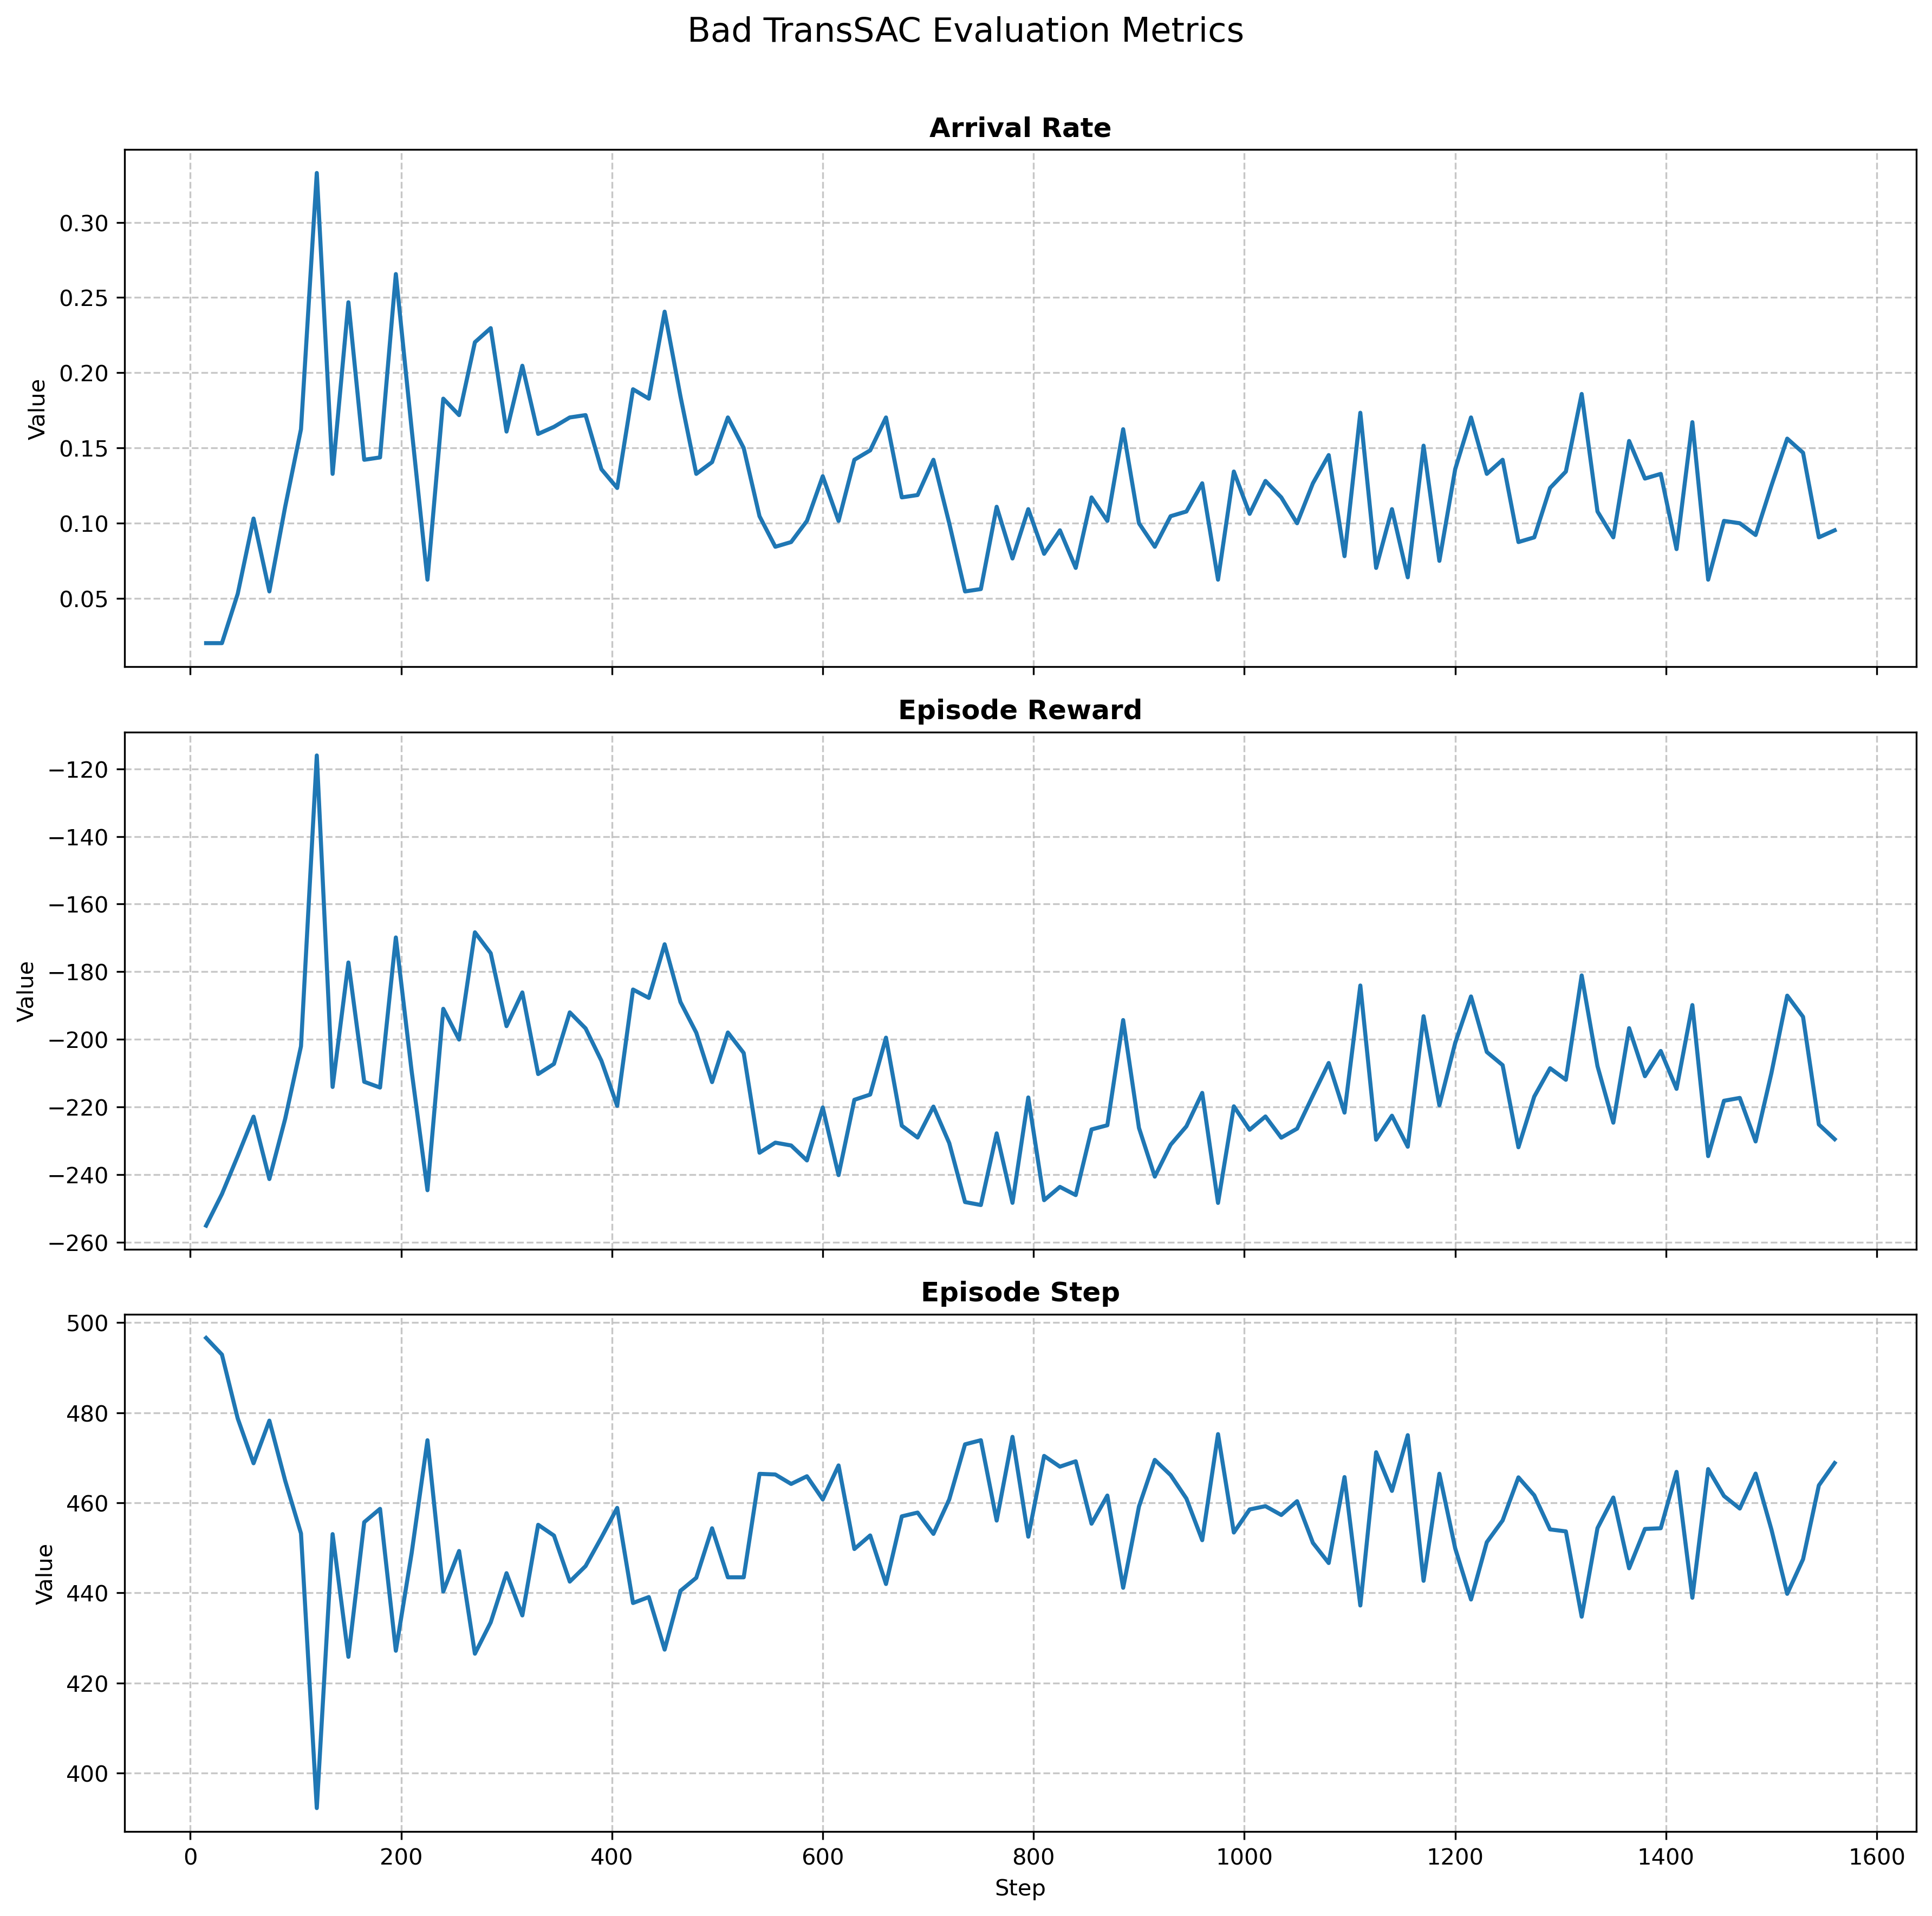
\includegraphics[width=0.7\textwidth,height=0.35\textheight,keepaspectratio]{figures/bad_transSAC/bad_transSAC_eval_combined.png}
    \caption{TransSAC 训练中策略网络崩塌评估结果}
    \label{fig:transSAC-eval-bad}
\end{figure}

如图 \ref{fig:transSAC-train-bad} 与图 \ref{fig:transSAC-eval-bad} 所示，
TransSAC模型面临着在早期培训阶段政策网络崩溃的明显挑战。在训练期间，演员的奖励曲线显示出巨大的波动，并在几千步内急剧下降到接近零。此行为表明策略网络未能学习有意义的操作分布。因此，智能体的行动退化为无效的随机探索。评估结果还显示，在早期训练期间，智能体达到目标的成功率保持在0\%到20\%之间的低水平。累积奖励也很低。这些结果进一步证实，策略崩溃对模型的导航性能有强烈的负面影响。

鉴于Transformer架构对序列中的离群值的敏感性以及非政策强化学习的训练动态，政策崩溃的可能原因分为以下三个维度。

\begin{enumerate}
    \item 爆炸性和高度波动的Q网络损失：Critic网络（损失/Q）的损失超过300，并强烈振荡。这意味着Q网络不能很好地匹配时间差目标（TD目标）。这个问题通常源于环境中的奖励量表太大、学习率设置过高或缺乏梯度剪切机制。
    \item Actor网络损失的持续增加：在SAC算法框架中，Actor的优化目标是最大化Q值和策略熵的总和，即$\alpha \log(\pi) - Q$。由于Q值发散和崩溃，演员的损失以不正常的方式上升。渐变的引导完全丢失了。
    \item 负奖励陷阱：平均训练奖励（训练/平均奖励）保持负值，完成率（训练/完成率）接近零。这表明智能体不断触发惩罚机制，例如与障碍物碰撞。该智能体属于局部次优政策，无法收集正奖励样本。
\end{enumerate} 

由于本研究中的模型使用Transformer结构，自我注意机制内的连乘法操作对序列特征的异常变化非常敏感。 如果在强化学习中没有将严格的梯度剪切应用于批评网络，或者如果批次大小不足以平滑序列特征分布，反向传播过程中的TD错误很容易导致梯度爆炸。

基于上述分析，本研究首先对Transformer网络架构应用了轻量化维减少处理。 采用单层编码器（$L=1$）和四个注意头（$H=4$）的基本配置。 这降低了最初的安装难度。 与此同时，为批评者网络单独设置了小学习率（$\mathrm{lr}_{\mathrm{critic}}=5 \times 10^{-5}$）。 这有助于压平早期训练阶段的极端梯度波动。 密切监控批评和TD误差分布的损失曲线，以确保它们保持在合理的范围内。

为了进一步确保模型在复杂的连续状态空间中稳定收敛，在算法的工程实现层面引入了一组训练稳定性机制。 这些机制描述如下：

\begin{enumerate}

\item 基于渐进式环境复杂性的课程学习：代理在冷启动阶段面临非常高的探索障碍。为了解决这个问题，引入了“婴儿步”渐进式课程学习机制。在总训练步骤的前15\%中，系统会动态调整环境配置。障碍物密度和动态难度逐步增加。这一策略可以防止策略崩溃，否则在早期阶段频繁的高处罚会导致策略崩溃。它还引导模型安全地度过脆弱的随机探索期。

\item 自适应梯度裁剪机制：梯度爆炸经常发生在深层网络和Transformer的自注意机制中。\cite{decision-transformer}为了抑制这个问题，在反向传播更新参数之前引入了全局梯度范数裁剪。根据每个模块的参数灵敏度设置不同的裁剪阈值。严格的裁剪标准（$max\_norm=0.5$）适用于高灵敏度的TransSAC主干网络。ASL分布式架构中的学习者模块使用较温和的阈值（$max\_norm=10$）。该机制限制了物理层面单个参数更新的最大步长。因此，优化路径保持平稳且可控。

\item 正交权重初始化：深度神经网络经常遭受梯度消失或特征方差转移。为了处理这个问题，使用正交矩阵来初始化线性层权重。缩放系数$\text{Gain} = \sqrt{2} \approx 1.414$设置为匹配ReLU激活函数系列。正交矩阵的规范在跨层信息传输期间保持梯度能量一致。这大大提高了深度网络的数值稳健性。在默认配置中，实验观察表明，$\alpha$值在复杂的环境分布下经历了不可逆的指数扩展。这迫使该政策退化为纯粹的随机行走。因此，目标熵的修正比例被保守地调整为0.6。这种选择锁定了$\alpha$参数收敛的上限，同时为必要的动作探索留有足够的空间。

\end{enumerate}

按上述流程逐项排查并调整，最终训练收敛。
\subsection{TransSAC算法评估分析}
评估结果如下：

\begin{figure}[H]
  \centering
  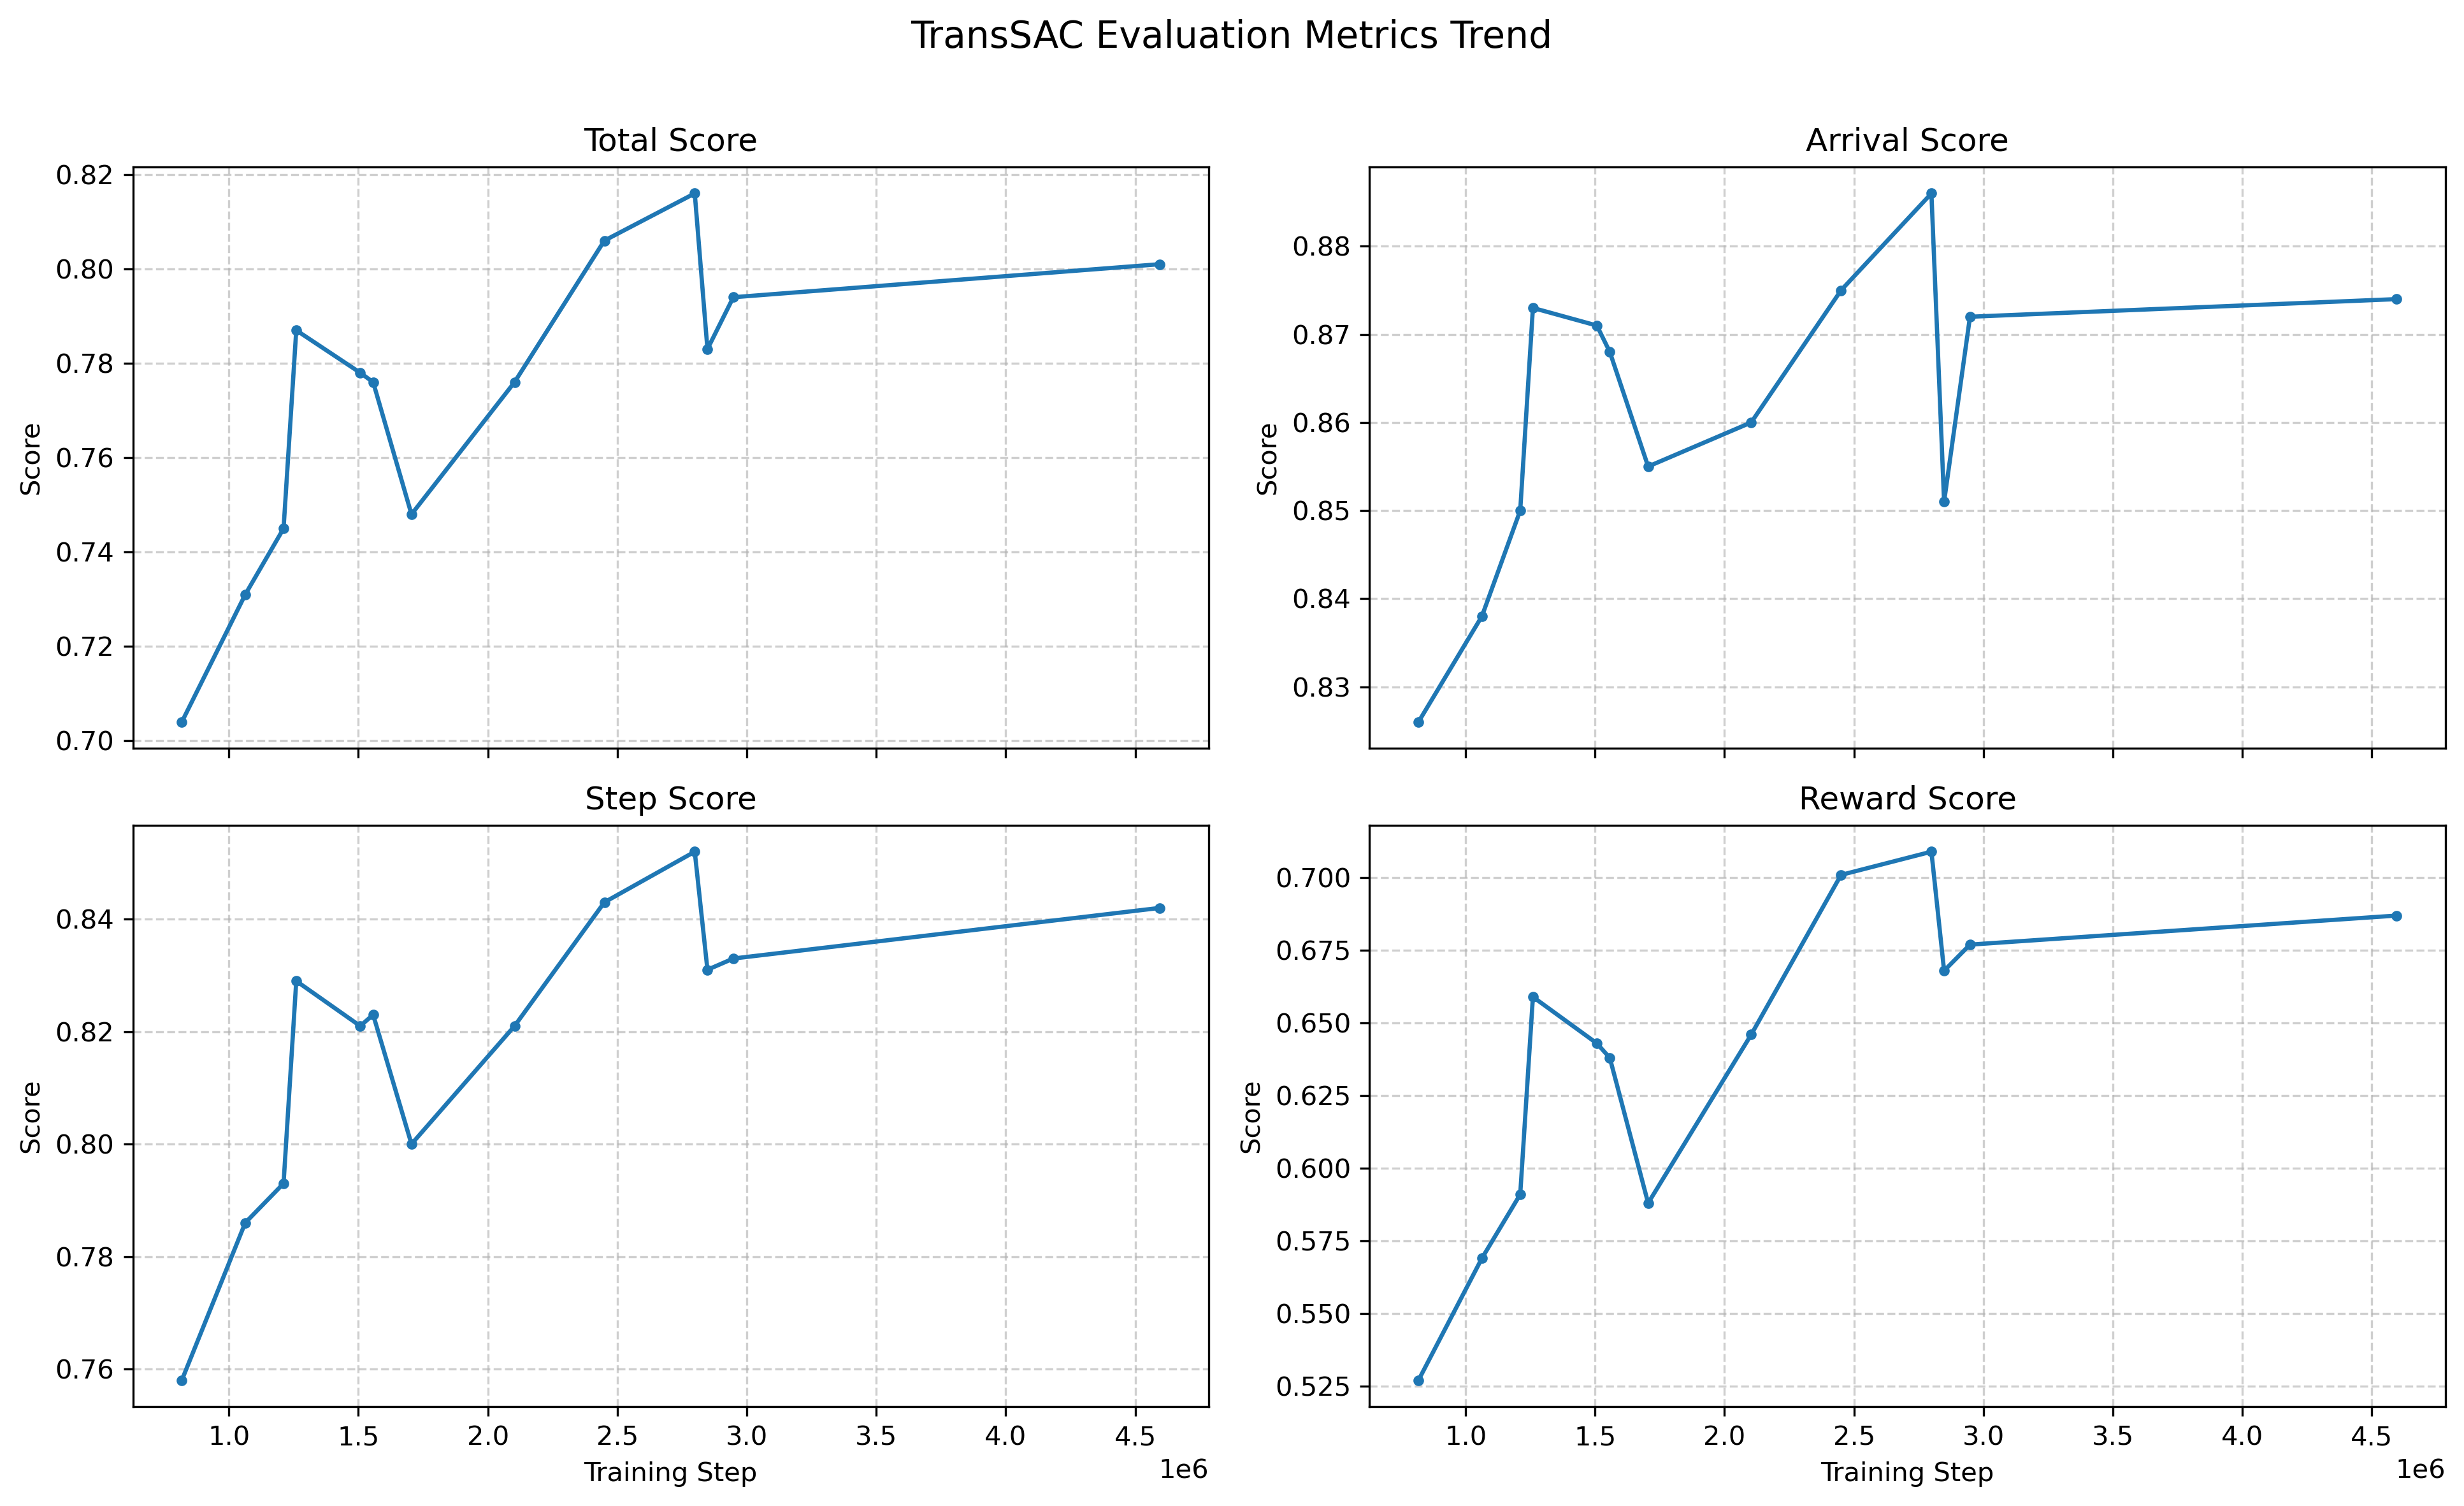
\includegraphics[width=0.7\textwidth]{figures/TransSAC_metrics_trend.png}
  \caption{TransSAC算法到达率、平均每回合步数和平均每回合奖励的训练趋势展示}
  \label{fig:transsac-showcase}
\end{figure}
从整体趋势的角度来看，培训过程波动很大。 尽管如此，所有指标（总分、到达分数、步数、奖励分数）在这些振荡中都显示出普遍上升趋势。 在训练接近尾声时，到达分数恢复并保持在0.87左右。 总分接近0.80。 这种行为表明，TransSAC算法可以处理复杂的导航或控制任务，并最终能够以高成功率收敛到有效的政策。

与传统无模型强化学习算法中的平滑收敛曲线不同，TransSAC显示了明显的“崖状”性能下降，约 $1.5 \times 10^6$ 步与 $2.8 \times 10^6$ 步左右快速反弹。 这种现象主要来自算法中使用的Transformer注意机制。 在探索过程中，由于状态特征序列是多样化的，注意力权重的分布容易发生剧烈震荡。 当智能体遇到未知状态空间或过渡概率的突然变化时，价值网络的估计可能会过度拟合或暂时偏离。 这导致策略评估不准确。 然而，通过SAC算法的最大熵机制和软更新策略，模型可以在崩溃后快速自我纠正。 它重新获得了最佳策略梯度，并表现出强大的快速恢复能力。

通过查看步数分数和奖励分数的同步下降和恢复，可以看到这两个分数之间的高度正相关性。 这一观察意味着，当Transformer架构提取高维时空特征时，智能体对平衡路径长度和奖励非常敏感。 由于模型容量更大，网络在拟合复杂状态表示时需要更多的数据样本来微调，这是评估指标在培训过程中不稳定的主要原因。

总体而言，TransSAC在早期训练中用绝对的稳定性换取了对复杂顺序特征的更强的提取和表示能力。 它最终的高到达分数表明了该架构在处理需要长期记忆或复杂空间感知的任务方面的巨大潜力。

与普通SAC相比，TransSAC显示出更稳定的到达分数，即使在早期训练阶段，也约为50\%。 这一结果表明，时间建模确实提高了决策质量。 在以后的验证比较中，这种架构的优势将被更精确地衡量。

\begin{figure}[http]
  \centering
  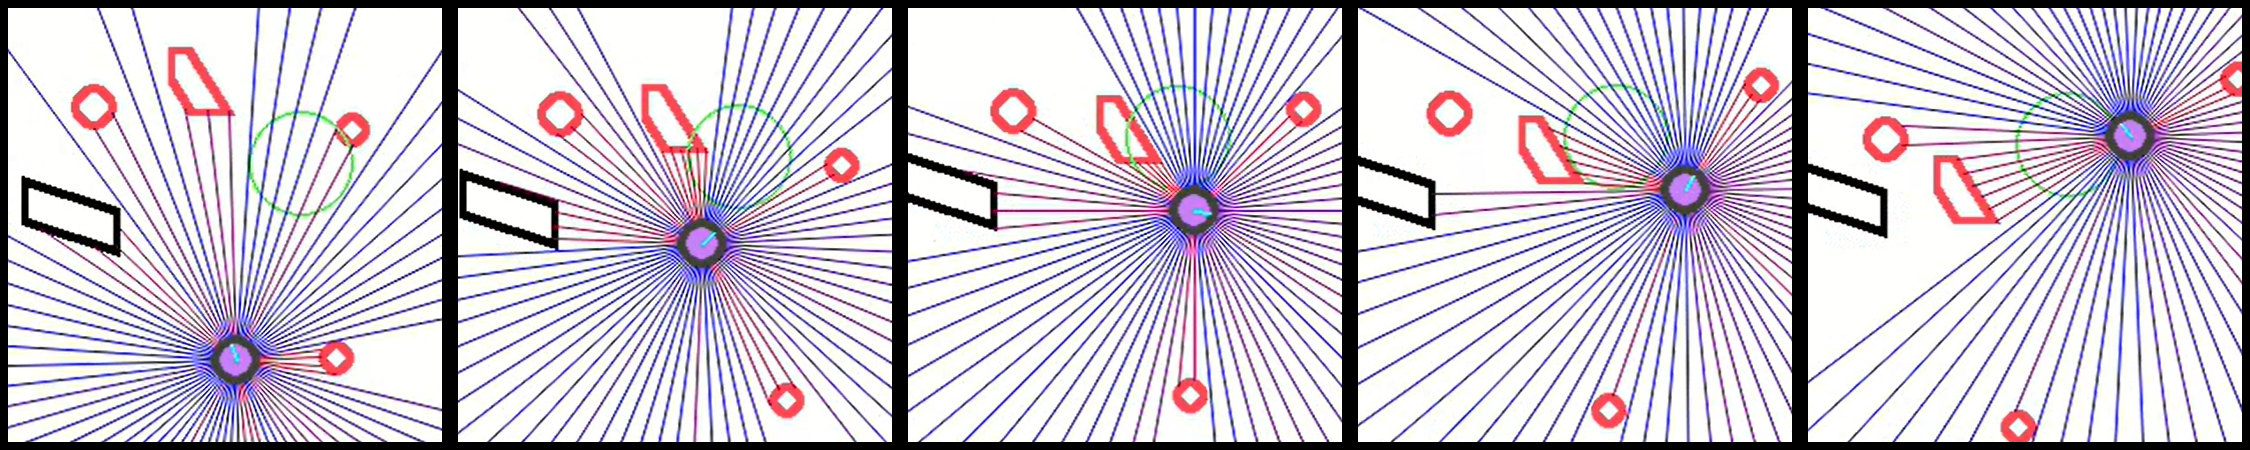
\includegraphics[width=0.7\textwidth]{figures/experiment1_stitched.png}
  \caption{TransSAC 训练中智能体学到的高级避障技能展示（序列1）}
  \label{fig:action_1}
\end{figure}

\begin{figure}[http]
  \centering
  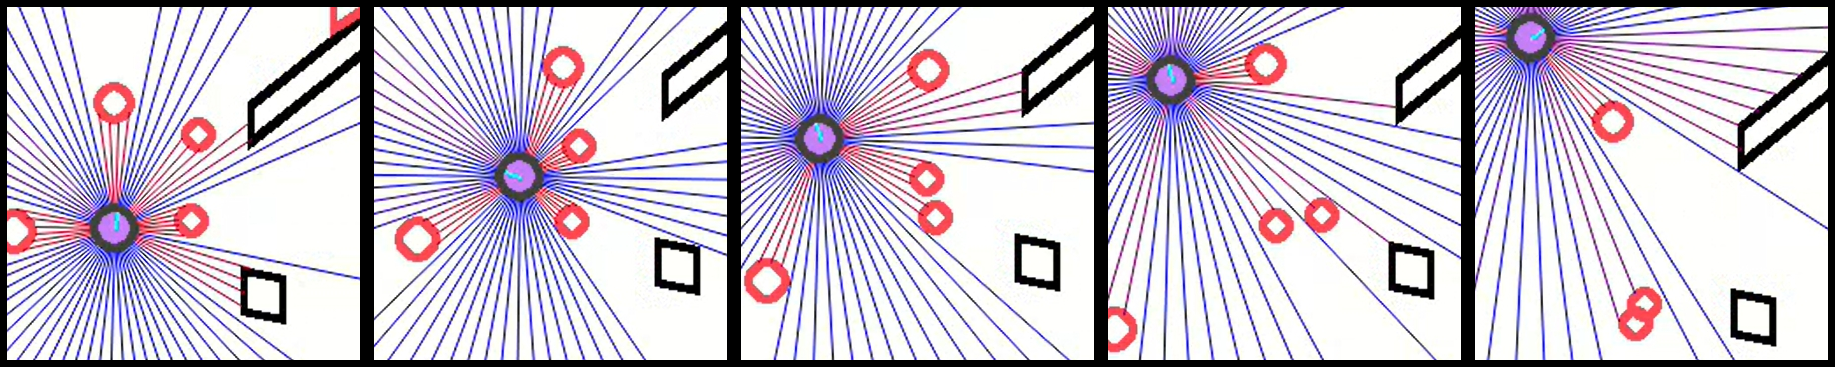
\includegraphics[width=0.7\textwidth]{figures/experiment2_stitched.png}
  \caption{TransSAC 训练中智能体学到的高级避障技能展示（序列2）}
  \label{fig:action_2}
\end{figure}

\begin{figure}[http]
  \centering
  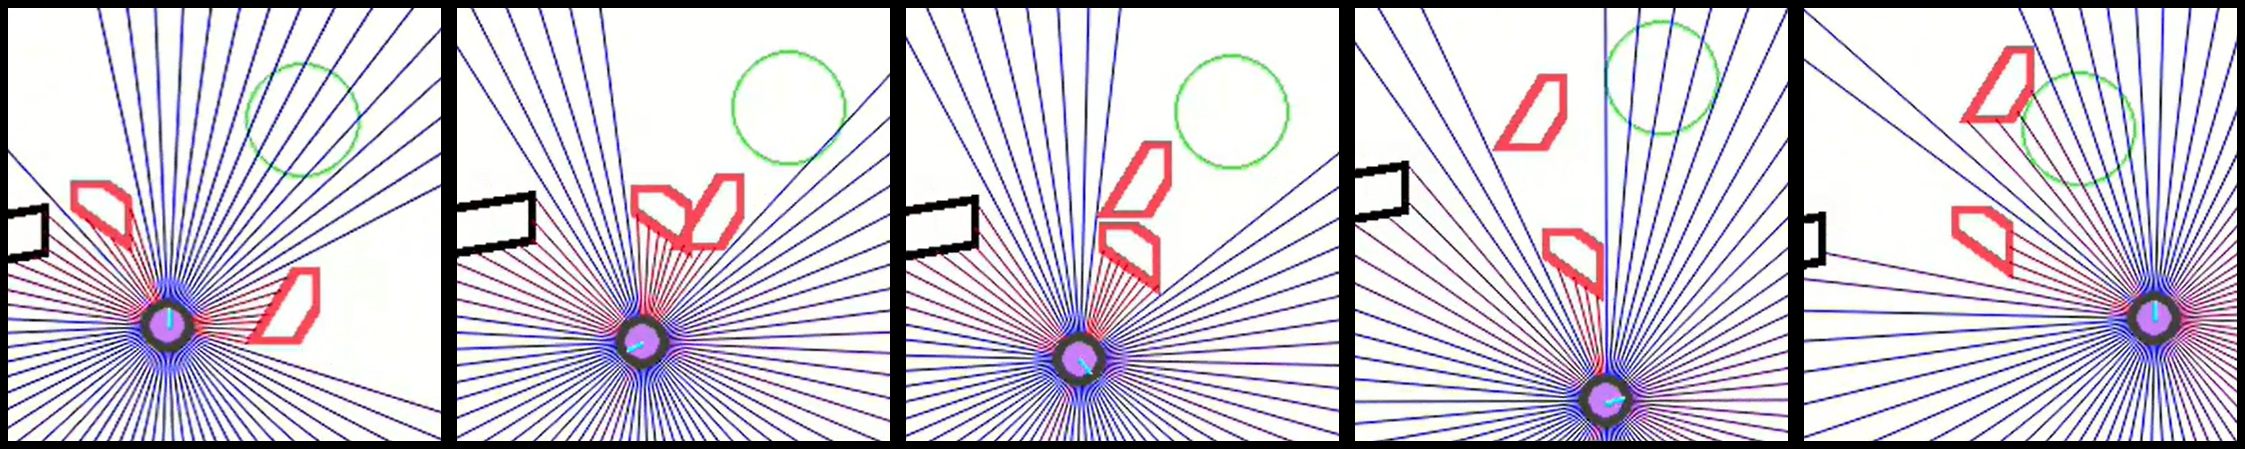
\includegraphics[width=0.7\textwidth]{figures/experiment3_stitched.png}
  \caption{TransSAC 训练中智能体学到的高级避障技能展示（序列3）}
  \label{fig:action_3}
\end{figure}
从上述实验序列可以看出，经过充分训练的 TransSAC 智能体学会了对动态障碍物的主动闪避、等待等在复杂环境中的路径优化的高级导航技能。
\section{路径规划算法对比}

为了全面评估所提出的算法在复杂导航场景下的有效性与优越性，本节开展了详细的比较研究。评估过程主要分为两个维度：首先，将经典的局部路径规划器（DWA）与基于深度强化学习的算法进行基准对比；其次，在强化学习框架内部，对主流的 DQN、SAC\_ASL 算法与本研究提出的 TransSAC 算法进行横向性能剖析。评估的核心指标包括模型训练过程中的到达率（Arrival Rate）、累积奖励（Cumulative Reward）以及任务步数/路径长度（Episode Steps）。

对于DWA经典算法，测试结果如下：
\begin{table}[http]
    \centering
    \caption{DWA经典算法测试结果}
    \label{tab:dwa_eval_result}
    \begin{tabular}{lcccc}
        \toprule
        \textbf{Index} & \textbf{Total Score} & \textbf{Arrival Score} & \textbf{Step Score} & \textbf{Reward Score} \\
        \midrule
        DWA & 0.304 & 0.53 & 0.442 & -0.06 \\
        \bottomrule
    \end{tabular}
\end{table}

对于强化学习算法，不同训练轮数的模型表现如下：
\begin{figure}[http]
  \centering
  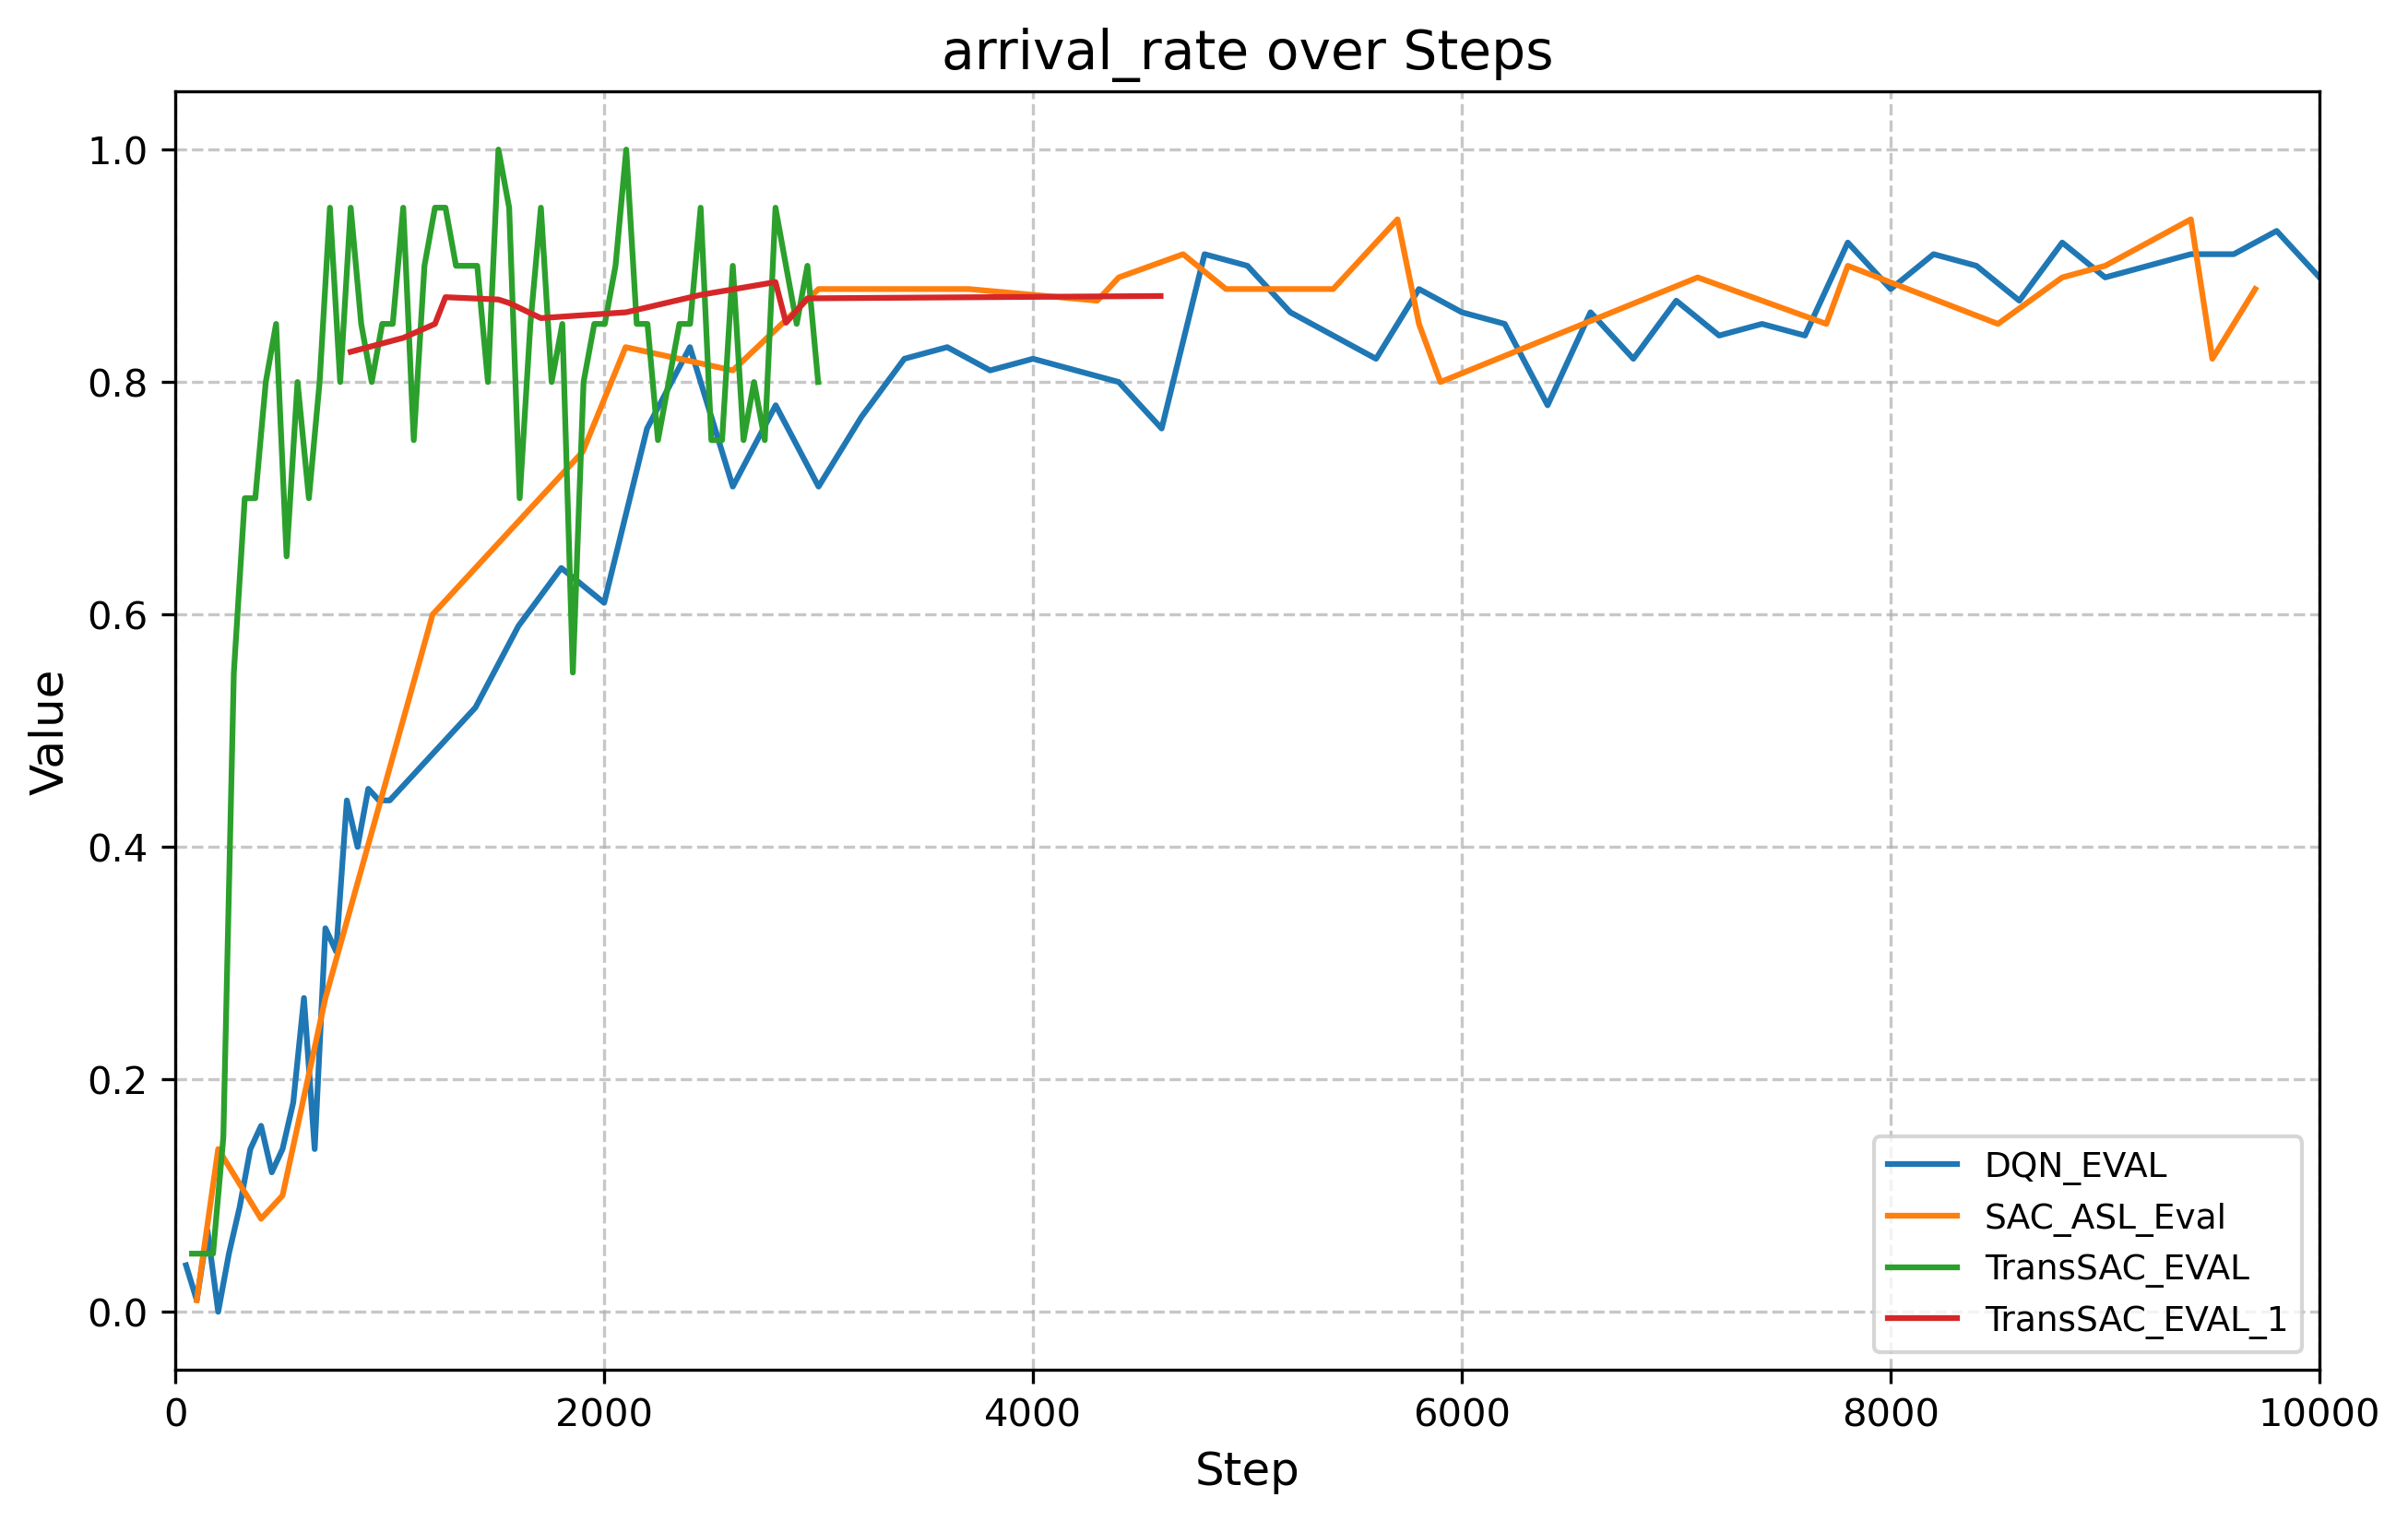
\includegraphics[width=0.7\textwidth]{figures/comparison/arrival_rate.png}
  \caption{到达率对比}
  \label{fig:comparison_arrival_rate}
\end{figure}
\begin{figure}[http]
  \centering
  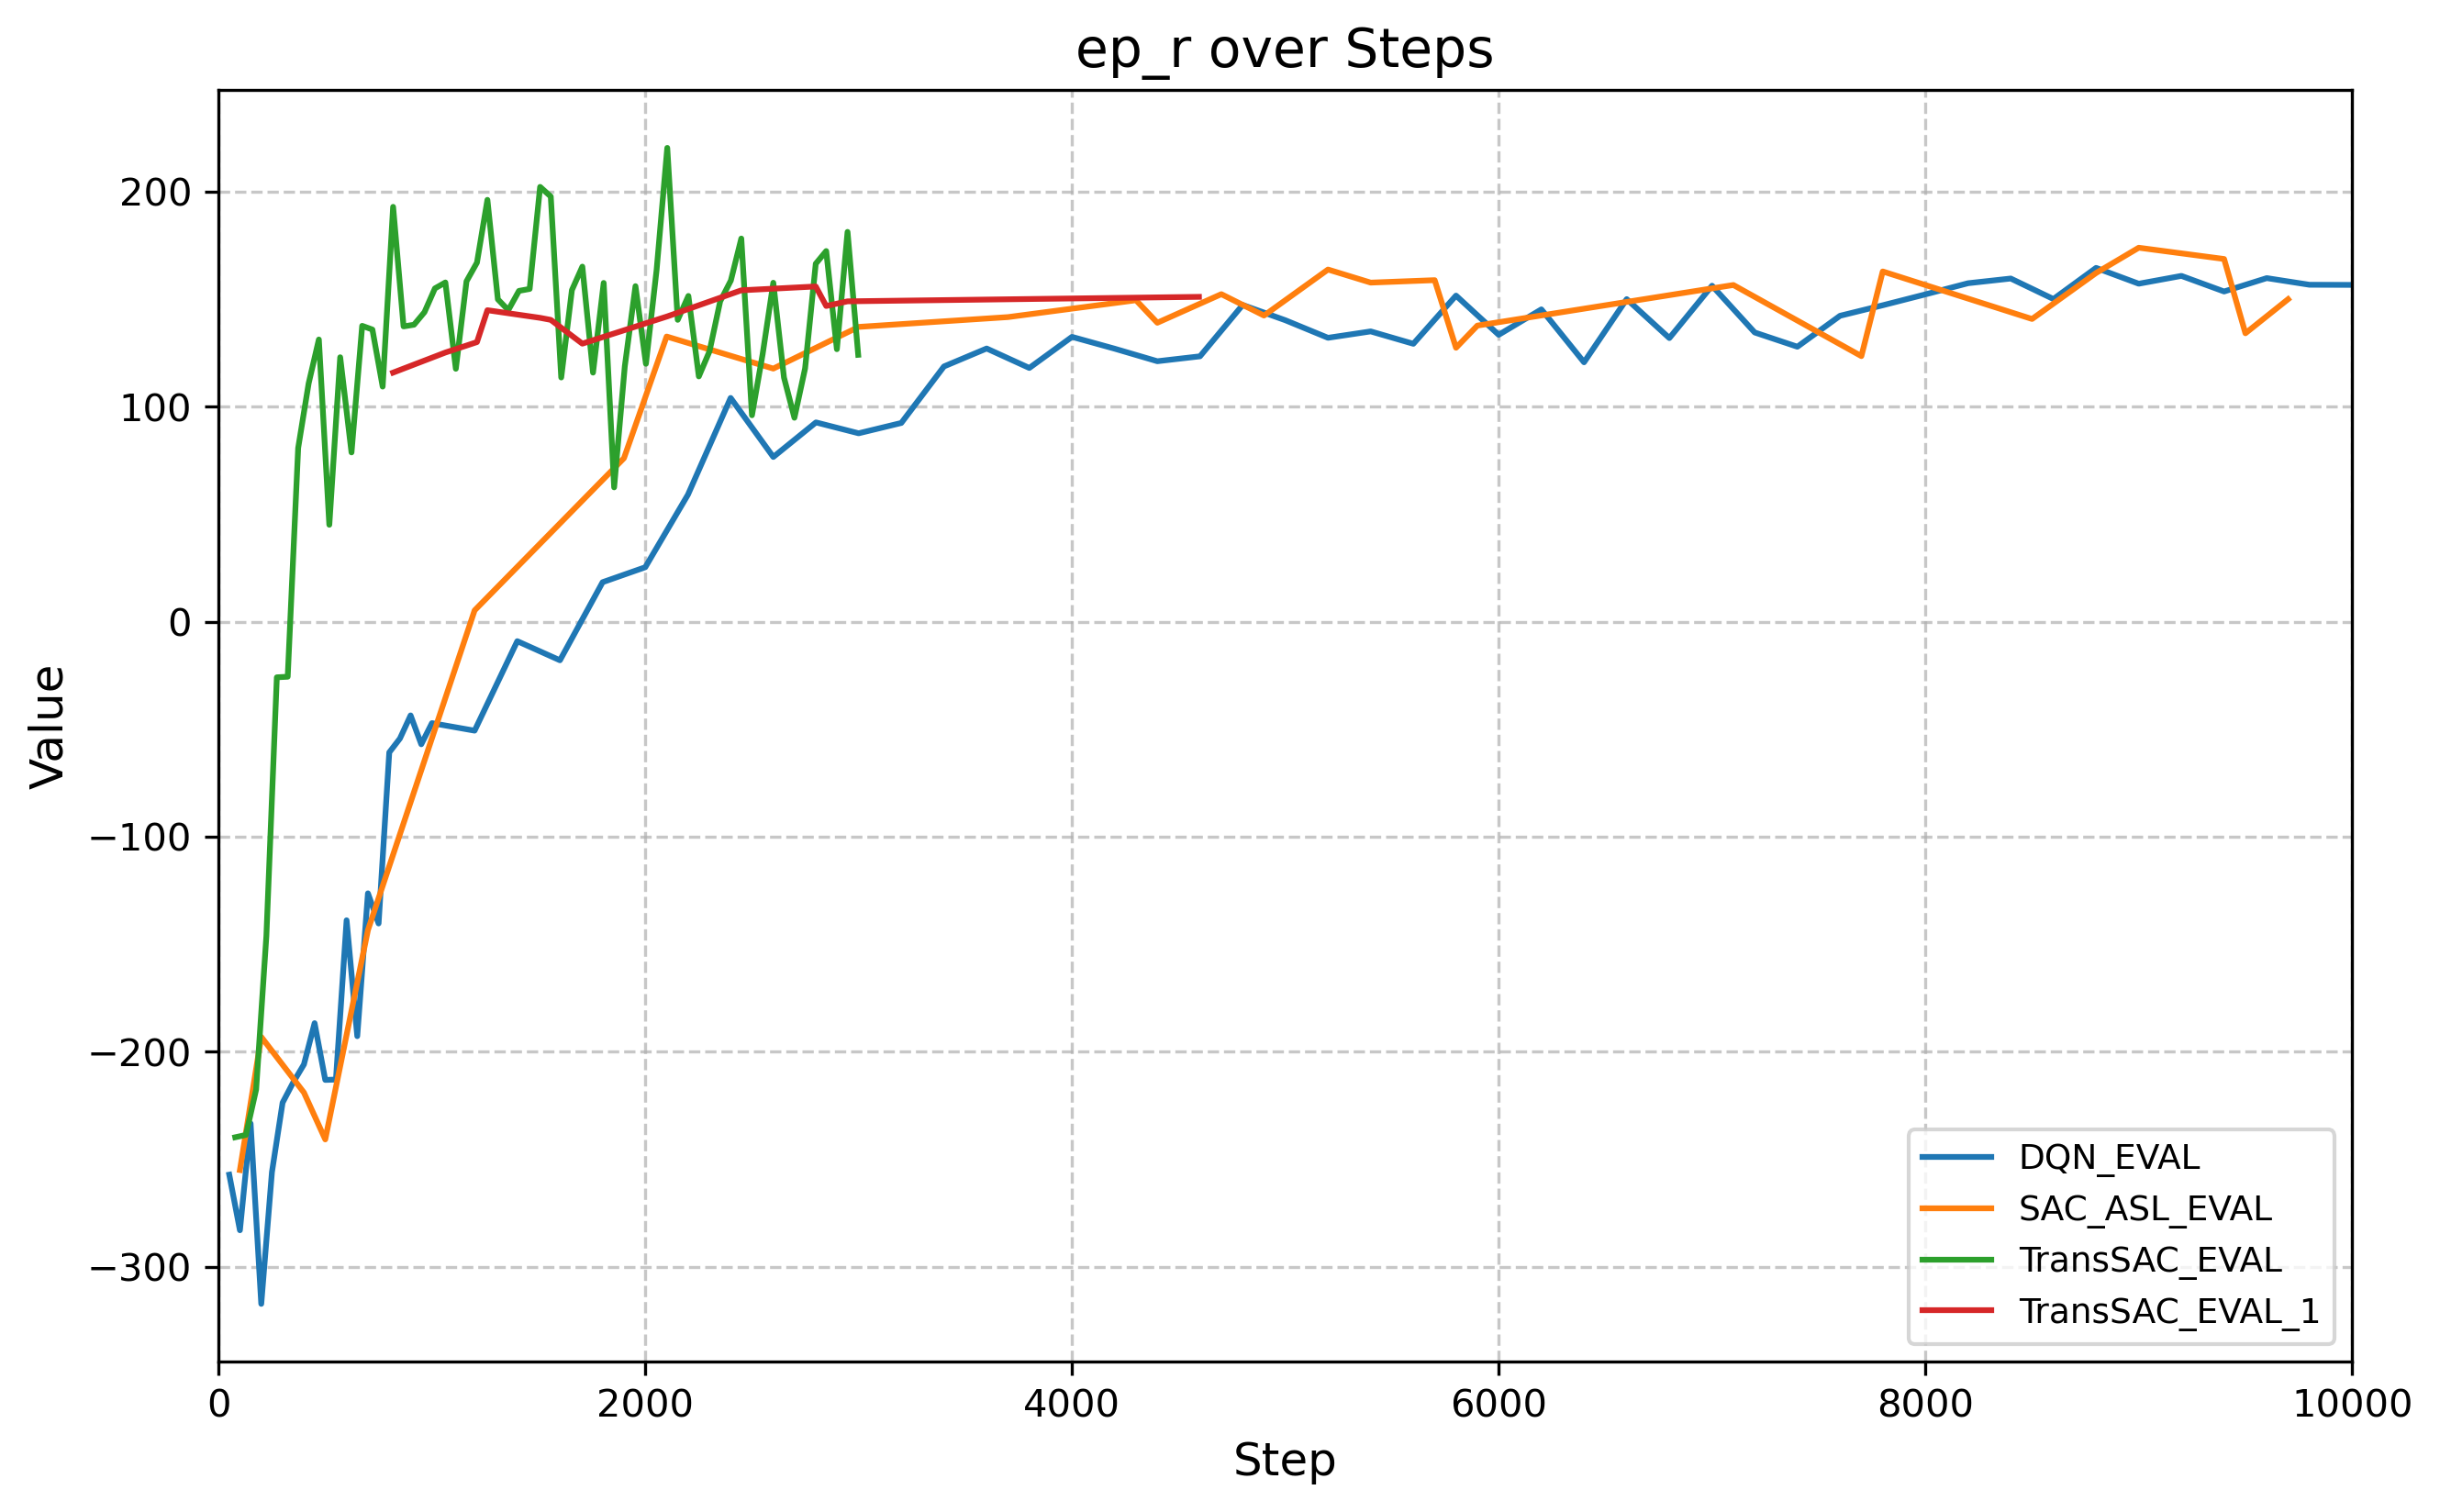
\includegraphics[width=0.7\textwidth]{figures/comparison/ep_r.png}
  \caption{累积奖励对比}
  \label{fig:comparison_ep_r}
\end{figure}
\begin{figure}[http]
  \centering
  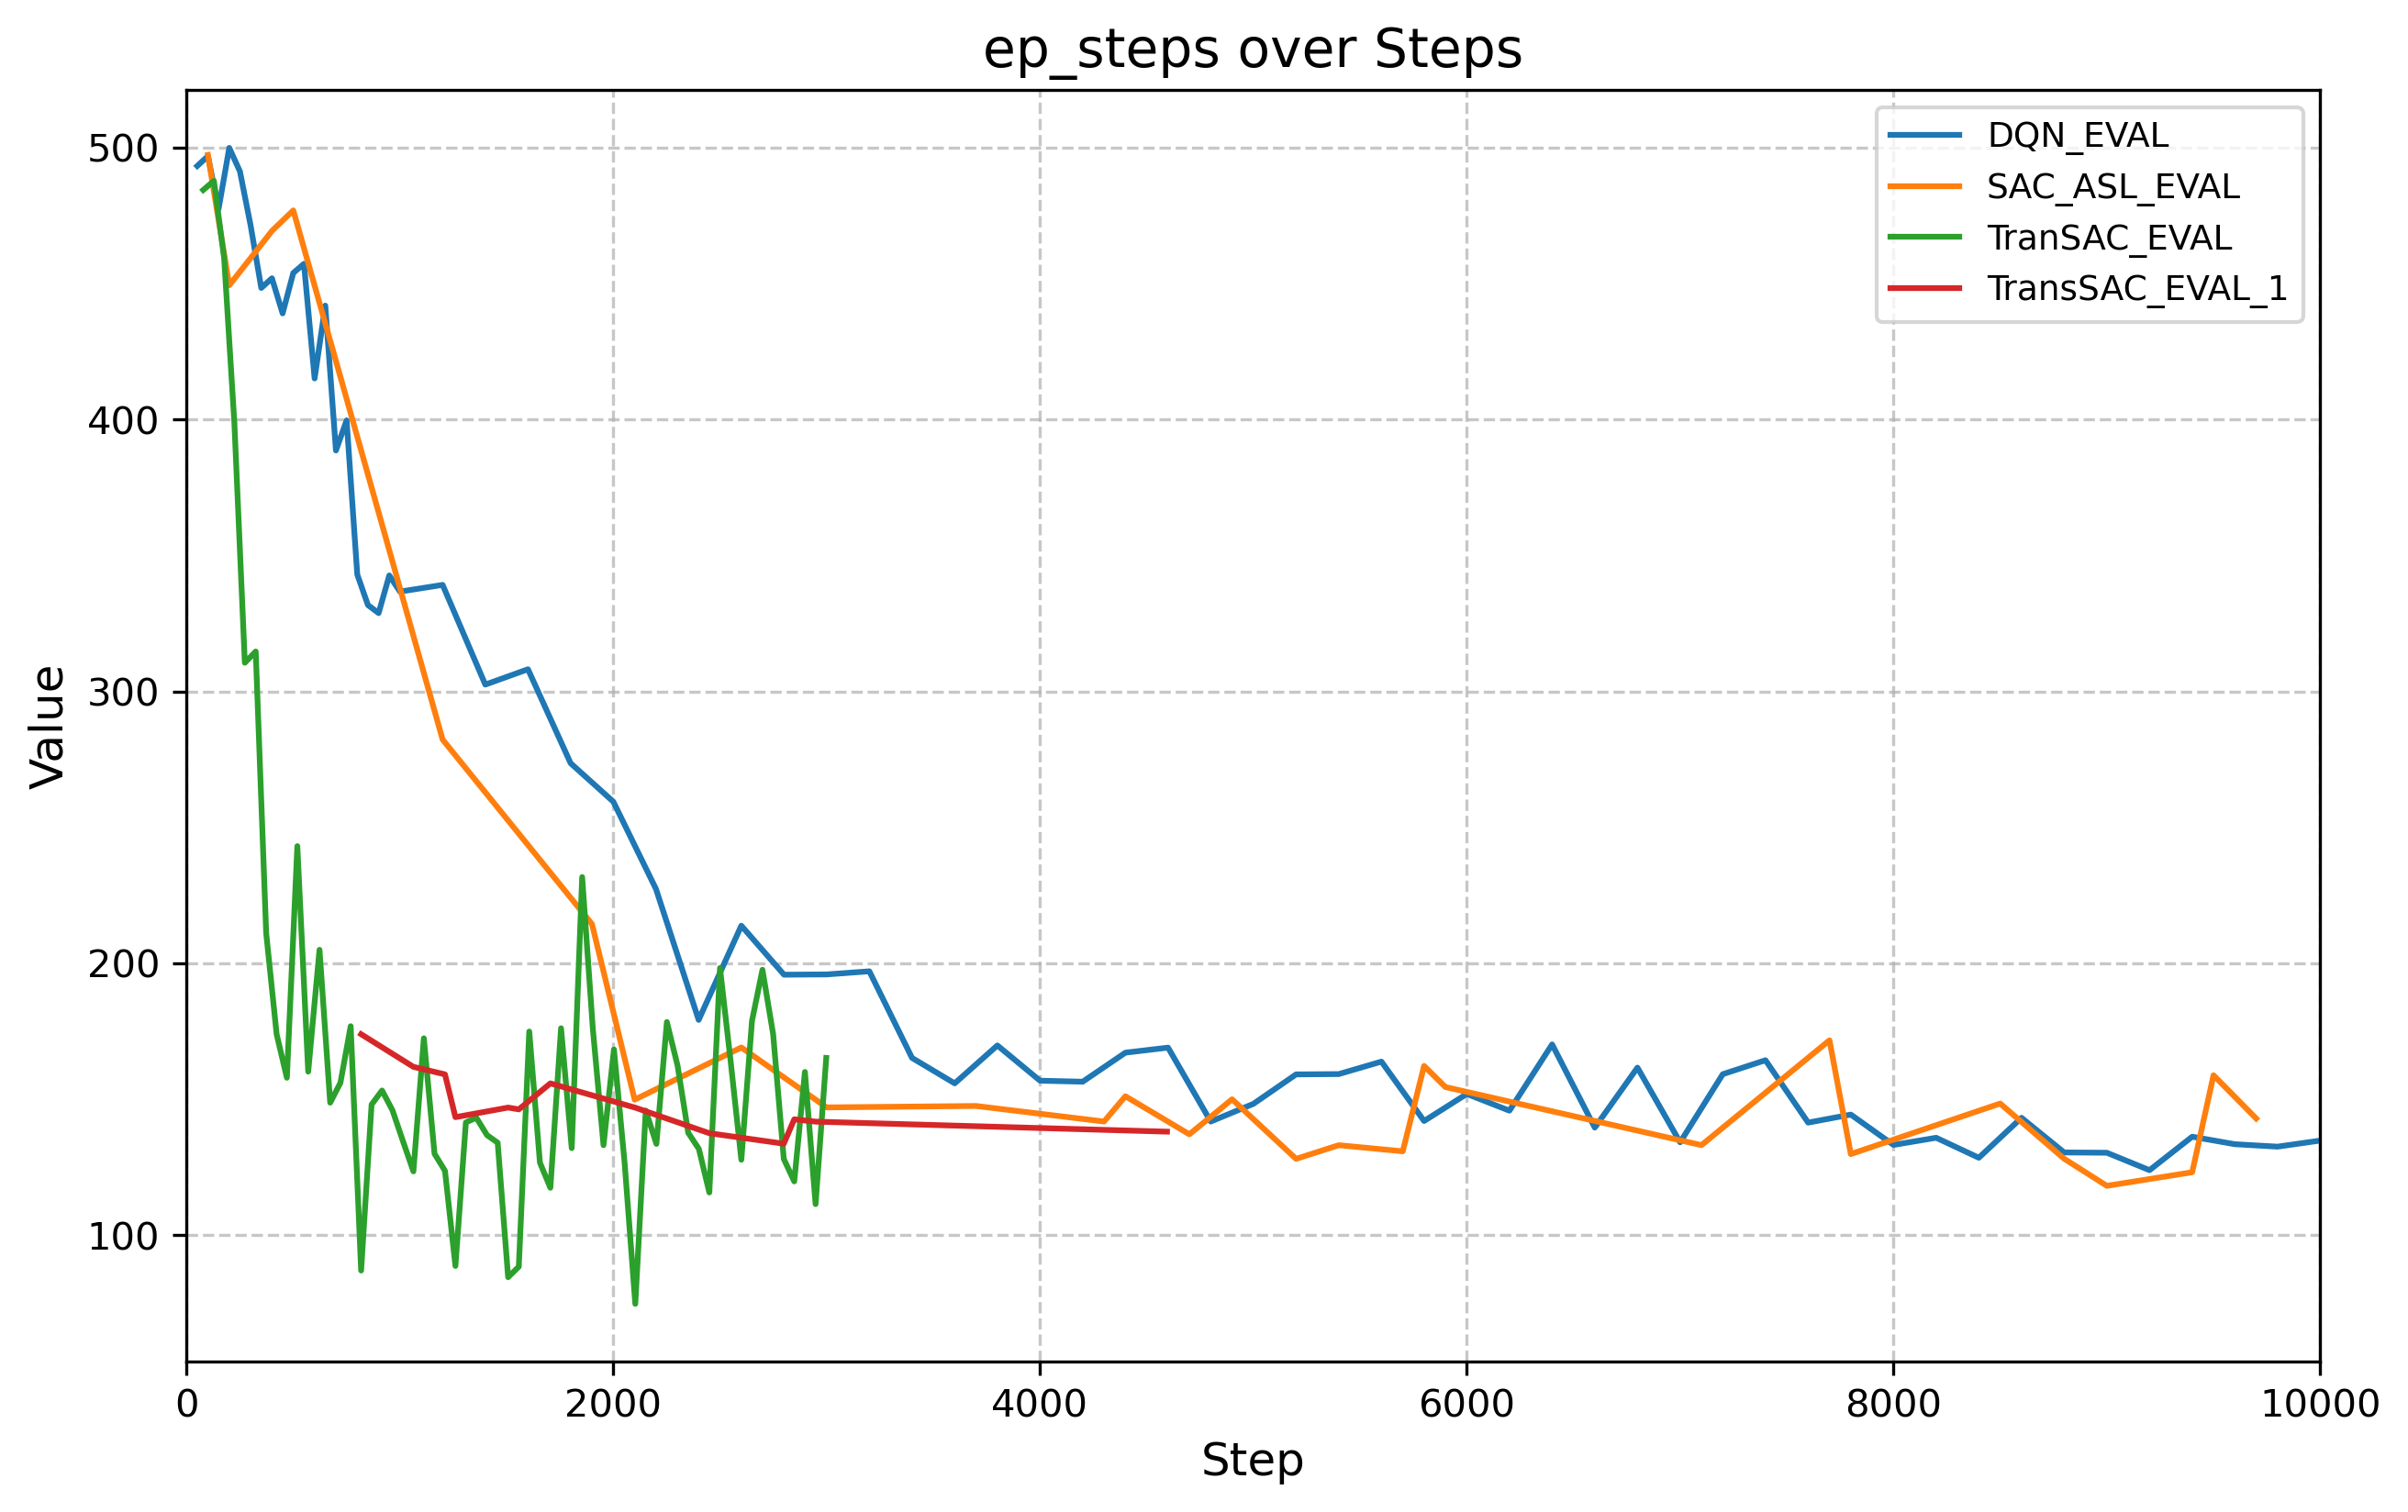
\includegraphics[width=0.7\textwidth]{figures/comparison/ep_steps.png}
  \caption{路径长度对比}
  \label{fig:comparison_ep_steps}
\end{figure}
\begin{table}[http]
    \centering
    \caption{三种路径规划算法综合性能对比}
    \label{tab:algo_comparison}
    \begin{tabular}{lcccc}
        \toprule
        \textbf{算法} & \textbf{综合评分} & \textbf{到达率} & \textbf{步数评分} & \textbf{奖励评分} \\
        \midrule
        DWA      & 0.304 & 0.530 & 0.442 & $-$0.060 \\
        DQN      & 见图~\ref{fig:dqn-showcase}     & —     & —     & — \\
        SAC      & 见图~\ref{fig:sac-showcase}     & —     & —     & — \\
        TransSAC & 见图~\ref{fig:transsac-showcase} & —     & —     & — \\
        \bottomrule
    \end{tabular}
\end{table}

\subsection{经典路径规划算法与深度强化学习算法比较}
为了展示数据驱动方法在复杂动态环境中的优势，本研究首先将其性能与传统动态窗口方法（DWA）的结果进行了比较。如表\ref{tab:dwa_eval_result}所述，结果表明，经典的DWA算法在几个导航指标上有明显的局限性。具体来说，DWA算法的到达分数仅为0.53。这意味着，在复杂的测试场景中，算法只有大约50\%的时间能成功到达到目标。它的奖励分数仅-0.06，步数分数仅0.442。

图\ref{fig:comparison_arrival_rate}与\ref{fig:comparison_ep_steps}中强化学习算法的收敛结果的比较表明，深度强化学习模型在成功率和路径优化方面都取得了巨大的收益。传统DWA算法的性能不佳主要是由于它严重依赖手动设置的成本函数权重。另一个原因是DWA只能在当前速度窗口内执行局部最佳采样。当面对U形障碍或高度动态的环境时，DWA往往会陷入局部最小值，这阻止了规划向前推进。相比之下，深度强化学习算法在许多场景中通过反复试验学习更多的高级避障策略。这有助于克服传统路径规划的有限视野固有限制。

\subsection{基于深度强化学习的算法内部性能比较}
为了进一步展示使用Transformer架构带来的强化学习性能的提高，本节比较了相同训练条件下的DQN、SAC和TransSAC算法。

\subsubsection{收敛速度和到达率：}

图\ref{fig:comparison_arrival_rate}中的到达率比较曲线显示了算法之间收敛行为的明显差异。 TransSAC（绿色和红色曲线表示）收敛得非常快。 经过大约1000个训练步后，它的到达率迅速上升，并保持在0.8以上。 它最终收敛到约0.9左右的高值。 传统的SAC\_ASL算法（橙色曲线）最终达到类似的成功率，但其收敛速度较慢。 稳定下来大约需要6000步。 DQN算法（蓝色曲线）表现最差。 它的勘探效率在早期阶段很低，后来会出现明显的性能波动。 TransSAC的这一优势主要来自添加到网络结构中的变压器模块。 该模块中的自我注意机制可以很好地处理时间传感器数据，加快了对环境动态障碍物的策略学习。

\subsubsection{长期政策和奖励获取：}
图 \ref{fig:comparison_ep_r} 显示了训练期间累积奖励的趋势。 随着训练的进行，所有三种算法的累积奖励都会上升。 这意味着算法的奖励函数设计是合理有效的。 然而，TransSAC模型可以在训练的早期阶段迅速离开负奖励区域。 它还在后期保持最高的平均累积奖励。 这一发现证实，TransSAC网络不仅提高了到达目标的概率，而且还能做出更好的决策来避免碰撞和保持安全距离。 DQN算法显示出最慢的逐步改进，并且之后有明显的波动。 这些结果表明，TransSAC具有更强的时间序列感知能力，可以更准确地预测动态障碍物的移动路径，规划更顺畅、更高效的几乎全局最佳路径。

\subsubsection{路径效率与规划寻优：} 导航路径的长度是衡量规划效率的关键指标，在此实验中对应衡量指标为\texttt{ep\_steps}。如图\ref{fig:comparison_ep_steps} 的任务步数对比所示，在训练初期，由于处于随机探索阶段，各算法的步数均处于 400 步以上，表明个算法均未学习到高效策略。随着训练步数增长模型收敛，TransSAC 的步数下降最迅速，并在 2000 步左右率先收敛至 150 步附近的极小值。DQN 算法的步数下降最慢，且后期震荡较大。这一结果表明，TransSAC 能够更好地预测动态障碍物的运动轨迹，从而为智能体规划出更加高效的运动路径。

综上所述，对比实验的结果有力地证明了 TransSAC 算法在复杂路径规划任务中的优越性。它不仅相较于经典 DWA 算法不会陷入局部最优的瓶颈，而且在收敛速度和路径最优性方面均优于传统强化学习算法 DQN 与 SAC 算法。

\section{实际电缆场景适应性分析}

电缆通道本质上属于典型的狭长有限空间作业场景，其物理环境具有较强约束性。结合本文前述分析，常规电缆通道的净宽一般约为0.8m至1.2m，净高一般约为1.2m至1.8m，内部除了电缆支架、转角、接线盒等静态构件外，还可能存在局部台阶、凸起和临时堆放物等障碍，其中局部凸起高度通常在0.2m至0.3m范围内。与此同时，实际巡检过程中还可能出现人员临时进入、推车移动等动态干扰，因此机器人不仅要具备稳定通过狭窄区域的能力，还需要具备对静态障碍物和动态障碍物的联合避让能力。

本章路径规划实验结果可以看出，DWA、DQN、SAC 和 TransSAC 分别对应了不同层次的导航能力，其中传统 DWA 在复杂动态环境中容易陷入局部最优，而基于强化学习的方法能够逐步学习更符合通道场景的避障与通行策略。特别是 TransSAC 在引入时序上下文后，能够更好地感知障碍物运动趋势和通道空间变化，在到达率、累积奖励以及路径长度等指标上表现更优。这表明该方法不仅能够在仿真环境中完成点到点导航，还能够适应电缆通道中“狭窄空间 + 局部障碍 + 动态干扰”并存的实际工况。

综上，本文所采用的控制与路径规划算法在物理参数约束、障碍通过能力以及动态避障能力三个方面都与实际电缆通道检测任务的需求相匹配，能够为机器人在真实电缆通道中的自主巡检提供可行的技术支撑。
